% Options for packages loaded elsewhere
\PassOptionsToPackage{unicode}{hyperref}
\PassOptionsToPackage{hyphens}{url}
\PassOptionsToPackage{dvipsnames,svgnames,x11names}{xcolor}
%
\documentclass[
  12pt,
]{article}

\usepackage{amsmath,amssymb}
\usepackage{setspace}
\usepackage{iftex}
\ifPDFTeX
  \usepackage[T1]{fontenc}
  \usepackage[utf8]{inputenc}
  \usepackage{textcomp} % provide euro and other symbols
\else % if luatex or xetex
  \usepackage{unicode-math}
  \defaultfontfeatures{Scale=MatchLowercase}
  \defaultfontfeatures[\rmfamily]{Ligatures=TeX,Scale=1}
\fi
\usepackage{lmodern}
\ifPDFTeX\else  
    % xetex/luatex font selection
\fi
% Use upquote if available, for straight quotes in verbatim environments
\IfFileExists{upquote.sty}{\usepackage{upquote}}{}
\IfFileExists{microtype.sty}{% use microtype if available
  \usepackage[]{microtype}
  \UseMicrotypeSet[protrusion]{basicmath} % disable protrusion for tt fonts
}{}
\makeatletter
\@ifundefined{KOMAClassName}{% if non-KOMA class
  \IfFileExists{parskip.sty}{%
    \usepackage{parskip}
  }{% else
    \setlength{\parindent}{0pt}
    \setlength{\parskip}{6pt plus 2pt minus 1pt}}
}{% if KOMA class
  \KOMAoptions{parskip=half}}
\makeatother
\usepackage{xcolor}
\setlength{\emergencystretch}{3em} % prevent overfull lines
\setcounter{secnumdepth}{5}
% Make \paragraph and \subparagraph free-standing
\ifx\paragraph\undefined\else
  \let\oldparagraph\paragraph
  \renewcommand{\paragraph}[1]{\oldparagraph{#1}\mbox{}}
\fi
\ifx\subparagraph\undefined\else
  \let\oldsubparagraph\subparagraph
  \renewcommand{\subparagraph}[1]{\oldsubparagraph{#1}\mbox{}}
\fi


\providecommand{\tightlist}{%
  \setlength{\itemsep}{0pt}\setlength{\parskip}{0pt}}\usepackage{longtable,booktabs,array}
\usepackage{calc} % for calculating minipage widths
% Correct order of tables after \paragraph or \subparagraph
\usepackage{etoolbox}
\makeatletter
\patchcmd\longtable{\par}{\if@noskipsec\mbox{}\fi\par}{}{}
\makeatother
% Allow footnotes in longtable head/foot
\IfFileExists{footnotehyper.sty}{\usepackage{footnotehyper}}{\usepackage{footnote}}
\makesavenoteenv{longtable}
\usepackage{graphicx}
\makeatletter
\def\maxwidth{\ifdim\Gin@nat@width>\linewidth\linewidth\else\Gin@nat@width\fi}
\def\maxheight{\ifdim\Gin@nat@height>\textheight\textheight\else\Gin@nat@height\fi}
\makeatother
% Scale images if necessary, so that they will not overflow the page
% margins by default, and it is still possible to overwrite the defaults
% using explicit options in \includegraphics[width, height, ...]{}
\setkeys{Gin}{width=\maxwidth,height=\maxheight,keepaspectratio}
% Set default figure placement to htbp
\makeatletter
\def\fps@figure{htbp}
\makeatother
\newlength{\cslhangindent}
\setlength{\cslhangindent}{1.5em}
\newlength{\csllabelwidth}
\setlength{\csllabelwidth}{3em}
\newlength{\cslentryspacingunit} % times entry-spacing
\setlength{\cslentryspacingunit}{\parskip}
\newenvironment{CSLReferences}[2] % #1 hanging-ident, #2 entry spacing
 {% don't indent paragraphs
  \setlength{\parindent}{0pt}
  % turn on hanging indent if param 1 is 1
  \ifodd #1
  \let\oldpar\par
  \def\par{\hangindent=\cslhangindent\oldpar}
  \fi
  % set entry spacing
  \setlength{\parskip}{#2\cslentryspacingunit}
 }%
 {}
\usepackage{calc}
\newcommand{\CSLBlock}[1]{#1\hfill\break}
\newcommand{\CSLLeftMargin}[1]{\parbox[t]{\csllabelwidth}{#1}}
\newcommand{\CSLRightInline}[1]{\parbox[t]{\linewidth - \csllabelwidth}{#1}\break}
\newcommand{\CSLIndent}[1]{\hspace{\cslhangindent}#1}

\usepackage{geometry}
\geometry{paper=a4paper,margin=1in}
\usepackage{fontspec}
\setmainfont{Arial}
\usepackage{ragged2e}
\usepackage{setspace}
\usepackage{parskip}
\setlength{\tabcolsep}{2pt}
\setlength{\parskip}{12pt}
\usepackage{float}
\floatplacement{figure}{H}
\usepackage{soul}
\makeatletter
\makeatother
\makeatletter
\makeatother
\makeatletter
\@ifpackageloaded{caption}{}{\usepackage{caption}}
\AtBeginDocument{%
\ifdefined\contentsname
  \renewcommand*\contentsname{Table of contents}
\else
  \newcommand\contentsname{Table of contents}
\fi
\ifdefined\listfigurename
  \renewcommand*\listfigurename{List of Figures}
\else
  \newcommand\listfigurename{List of Figures}
\fi
\ifdefined\listtablename
  \renewcommand*\listtablename{List of Tables}
\else
  \newcommand\listtablename{List of Tables}
\fi
\ifdefined\figurename
  \renewcommand*\figurename{Figure}
\else
  \newcommand\figurename{Figure}
\fi
\ifdefined\tablename
  \renewcommand*\tablename{Table}
\else
  \newcommand\tablename{Table}
\fi
}
\@ifpackageloaded{float}{}{\usepackage{float}}
\floatstyle{ruled}
\@ifundefined{c@chapter}{\newfloat{codelisting}{h}{lop}}{\newfloat{codelisting}{h}{lop}[chapter]}
\floatname{codelisting}{Listing}
\newcommand*\listoflistings{\listof{codelisting}{List of Listings}}
\makeatother
\makeatletter
\@ifpackageloaded{caption}{}{\usepackage{caption}}
\@ifpackageloaded{subcaption}{}{\usepackage{subcaption}}
\makeatother
\makeatletter
\@ifpackageloaded{tcolorbox}{}{\usepackage[skins,breakable]{tcolorbox}}
\makeatother
\makeatletter
\@ifundefined{shadecolor}{\definecolor{shadecolor}{rgb}{.97, .97, .97}}
\makeatother
\makeatletter
\makeatother
\makeatletter
\makeatother
\ifLuaTeX
  \usepackage{selnolig}  % disable illegal ligatures
\fi
\IfFileExists{bookmark.sty}{\usepackage{bookmark}}{\usepackage{hyperref}}
\IfFileExists{xurl.sty}{\usepackage{xurl}}{} % add URL line breaks if available
\urlstyle{same} % disable monospaced font for URLs
\hypersetup{
  pdftitle={Mapping India in Pliny the Elder's Natural History},
  pdfauthor={Dawn, Lizao Zhuang},
  pdfkeywords={Natural History, Pliny the Elder, Spatial
Humanities, Indo-Roman, Indo-Mediterranean},
  colorlinks=true,
  linkcolor={blue},
  filecolor={Maroon},
  citecolor={Blue},
  urlcolor={Blue},
  pdfcreator={LaTeX via pandoc}}

\title{Mapping India in Pliny the Elder's \emph{Natural History}}
\author{Dawn, Lizao Zhuang}
\date{}

\begin{document}

\maketitle
\thispagestyle{empty}

\newpage

\pagenumbering{Roman}
\setlength{\parskip}{12pt}
%----------------------------------------------
%   Preface
%----------------------------------------------

\raggedright

\Large\textbf{Preface}   

\vspace*{\baselineskip}
\normalsize
\justifying
This thesis aims to explore the first encyclopedia of the ancient world using digital methods within the scope of spatial humanities. Through a combination of skills acquired in the Digital Humanities programme - such as textual analysis, network analysis and data visualisation - and the integration of markup languages for interactive presentations, I have gained valuable training in conducting insightful digital humanities research.

Writing this thesis has been both an enjoyable journey through Pliny's encyclopaedic landscape and a fulfilling exploration of digital methods. Throughout this journey, I deeply appreciate the extensive guidance and help of my supervisor, Professor Margherita Fantoli, and my daily advisor, Laura Soffiantini. Professor Fantoli's constant reminder to ``have fun'' during classes, assignments, events, and feedback sessions encouraged me to tackle challenges and find joy in the process. Discussions with Laura were always enlightening; her inspiring instructions and technical mentorship have been invaluable to my progress.

Last but not least, I would like to thank my dear family and friends for their continuous care, understanding and sweet support.

\newpage


%----------------------------------------------
%   Abstract
%----------------------------------------------

\raggedright

\Large\textbf{Abstract}   

\vspace*{\baselineskip}
\normalsize
\justifying
This study examines Pliny's \textit{Natural History} from a spatial perspective, focusing on the content relating to India and incorporating the digitised and annotated text available in the \href{https://topostext.org/}{TOPOSText project}. The research employs a variety of methodologies, including word frequency and collocation analysis, topic modelling and network analysis, with an integration of close reading practices.
      
The multifaceted role that India plays in the narrative is highlighted in the study's findings. It emerges not only as a geographical counterpart and repository of precious treasures, but also as an important trading partner of the Roman Empire and the Mediterranean, a context closely related to Pliny's Stoic perspective on the natural world. In addition, the creation of a network map linking place and person names associated with India highlights the clustering of historical figures in the content structure.

\newpage

%----------------------------------------------
%   List of abbreviations
%----------------------------------------------

\raggedright

\Large\textbf{List of abbreviations}   

\vspace*{\baselineskip}
\normalsize
CSV: Comma-separated Values\\
\medskip
HTML: HyperText Markup Language\\
\medskip
LDA: Latent Dirichlet Allocation\\
\medskip
NER: Named Entity Recognition\\
\medskip
NLP: Natural Language Processing \\
\medskip
TOPOSText: \href{https://topostext.org/}{TOPOSText project} \\
\medskip
TXT: Text File\\
\medskip
XML: Extensible Markup Language\\

\newpage

\normalsize
\justifying\ifdefined\Shaded\renewenvironment{Shaded}{\begin{tcolorbox}[breakable, interior hidden, boxrule=0pt, borderline west={3pt}{0pt}{shadecolor}, enhanced, sharp corners, frame hidden]}{\end{tcolorbox}}\fi

\renewcommand*\contentsname{Table of Contents}
{
\hypersetup{linkcolor=}
\setcounter{tocdepth}{3}
\tableofcontents
}
\clearpage
\listoffigures
\listoftables
\setstretch{1.15}
\clearpage
\pagestyle{plain}
\pagenumbering{arabic}  
\setcounter{page}{1}

\hypertarget{sec-introduction}{%
\section{Introduction}\label{sec-introduction}}

\hypertarget{natural-history-and-its-complexity}{%
\subsection{\texorpdfstring{\emph{Natural History} and its
complexity}{Natural History and its complexity}}\label{natural-history-and-its-complexity}}

Pliny the Elder's \emph{Natural History} is widely recognized as the
earliest encyclopedia in the world, manifesting a pioneering effort in
comprehensively cataloguing the vast array of human knowledge from that
era.

The work is thematically divided into 37 books, covering a diverse range
of subjects including astronomy, geography, zoology, botany, medicine,
and more. Pliny meticulously consulted a wide range of Greek and Roman
references, totalling approximately 2,000 volumes\footnote{\emph{Natural
  History} 1.5.1 (https://topostext.org/work/148)}, and interwove his
own literary interpretation or comments to the narratives.

Despite the carefully designed knowledge-ordering framework (Lao 2016),
scholars have observed a paradoxical complexity in \emph{Natural
History}, evident in its linguistic style, narrative approach, and use
of references. The work compiles variant toponyms from Greek and Latin,
includes digressions in descriptions (Roller 2022), and exhibits changes
in vocabularies and sentence structures (Pinkster 2005). However, it is
precisely this complexity that makes the work more fascinating and not
only a valuable source of the knowledge and worldview of the ancient
world, but also a gateway into Pliny's conceptualization, imagination,
and even the prevailing imperial ideology of that time.

The complexity and interconnectivity of the general structure of
\emph{Natural History} are further highlighted in different aspects by
refreshing approaches. For the content organisation, Healy (1999)
advocated Pliny's original contribution in revealing the technology and
science engagement of the Rome Empire. Taking the historical, political
and linguistic context into consideration, he found that in addition to
providing informative descriptions of natural phenomena and scientific
experiments, Pliny also developed the scientific language in Latin
through his work. Moreover, Naas (2002) discussed how Pliny formulated
the diverse materials into his encyclopaedic structure, revealing the
work's multifaceted nature as an epistemological, ideological, and moral
project. Analysing Pliny's employment of the historical exemplum in the
work, Schultze (2011) argued how that literary device directed and
teased the readers as well as established a profound connection between
human beings and the entire spectrum of nature in \emph{Natural
History}.

In addition to the contextual and referential analyses of \emph{Natural
History}, Rydberg-Cox (2021) employed network analysis techniques,
applying various metrics to illustrate the connections between Pliny's
sources and the topics discussed in the work. Furthermore, Fantoli
(2022) conducted a comparative examination of book 2 of \emph{Natural
History} and book 7 of Seneca's \emph{Natural Questions}, both focused
on astronomy as part of the Latin classics about nature. Statistical
methods were applied to investigate variations in their discursive
distribution, effectively identifying Pliny's distinctive stylistic
attributes. Moreover, the encyclopaedic authorial intent evident in
\emph{Natural History} is validated through correspondence and tree
analysis. These studies collectively showcase how distant reading
methodologies offer novel insights into our understanding of ancient
treatises.

\hypertarget{spatial-perspective-in-natural-history}{%
\subsection{\texorpdfstring{Spatial perspective in \emph{Natural
History}}{Spatial perspective in Natural History}}\label{spatial-perspective-in-natural-history}}

As pointed out by Beagon (2011), differentiating from his predecessors,
Pliny showed a ``terrestrial curiosity'' in \emph{Natural History},
emphasising recognition of the physical, material world. In this regard,
the vision of geography plays a pivotal role in distributing
information, knowledge, and events throughout \emph{Natural History}.

Drawing from the long-established topographical and ethnographic
traditions, Pliny seamlessly connects volumes dedicated to geography
(books 3-6) with broader elements, activities, and cultural, historical,
and societal contexts(Roller 2022), exemplified in his portrayal of
exotic plants, communities' habitats, imperial expeditions, and trade
products. In other words, geographical names that occurred in each book
of \emph{Natural History} served as signposts guiding readers through
diverse lands, shedding light on how Pliny and his contemporaries
perceived and conceptualized the world around them.

A normalized frequency of place name occurrence in the work is
calculated as the ratio of counts of the occurrences of place names in
each book to the word lengths of the book
(Table~\ref{tbl-place_book_distribution}). The bar chart
(Figure~\ref{fig-place_distribution}) depicts the comparison of the
distribution of place names in the books of \emph{Natural History}. The
process of data collection and structuring for this table and chart is
further explained in the Methodology chapter
(Section~\ref{sec-methodology}).

The observation aligns with the content structure of \emph{Natural
History}, that books 3-6 centred around the themes of ``geography and
ethnography'', contain the most mentions of location names, and place
names are also frequently mentioned in books about agriculture and
horticulture (book 12-14), aquatic life (book 31), and mining and
mineralogy (book 34-37).

\hypertarget{tbl-place_book_distribution}{}
\begin{longtable}[]{@{}llll@{}}
\caption{\label{tbl-place_book_distribution}Normalized distribution of
place names in \emph{Natural History}}\tabularnewline
\toprule\noalign{}
& Total\_length & Place\_count & Place\_freq \\
Book & & & \\
\midrule\noalign{}
\endfirsthead
\toprule\noalign{}
& Total\_length & Place\_count & Place\_freq \\
Book & & & \\
\midrule\noalign{}
\endhead
\bottomrule\noalign{}
\endlastfoot
1 & 2778 & 1 & 0.000360 \\
2 & 30570 & 406 & 0.013281 \\
3 & 18037 & 1007 & 0.055830 \\
4 & 15434 & 1309 & 0.084813 \\
5 & 18872 & 1112 & 0.058923 \\
6 & 27891 & 1012 & 0.036284 \\
7 & 21204 & 225 & 0.010611 \\
8 & 24176 & 185 & 0.007652 \\
9 & 19197 & 140 & 0.007293 \\
10 & 20816 & 121 & 0.005813 \\
11 & 27345 & 77 & 0.002816 \\
12 & 13906 & 188 & 0.013519 \\
13 & 13243 & 164 & 0.012384 \\
14 & 15277 & 189 & 0.012372 \\
15 & 14552 & 135 & 0.009277 \\
16 & 25442 & 180 & 0.007075 \\
17 & 29387 & 82 & 0.002790 \\
18 & 35850 & 222 & 0.006192 \\
19 & 18822 & 146 & 0.007757 \\
20 & 22743 & 21 & 0.000923 \\
21 & 17896 & 95 & 0.005308 \\
22 & 16491 & 24 & 0.001455 \\
23 & 15764 & 17 & 0.001078 \\
24 & 17491 & 56 & 0.003202 \\
25 & 16734 & 85 & 0.005079 \\
26 & 15448 & 35 & 0.002266 \\
27 & 12444 & 40 & 0.003214 \\
28 & 26476 & 28 & 0.001058 \\
29 & 13976 & 31 & 0.002218 \\
30 & 14395 & 23 & 0.001598 \\
31 & 12204 & 222 & 0.018191 \\
32 & 14635 & 76 & 0.005193 \\
33 & 17946 & 113 & 0.006297 \\
34 & 18972 & 193 & 0.010173 \\
35 & 21283 & 277 & 0.013015 \\
36 & 21295 & 357 & 0.016764 \\
37 & 22255 & 282 & 0.012671 \\
\end{longtable}

\begin{figure}

{\centering \includegraphics{NHthesis_structure_files/figure-pdf/fig-place_distribution-output-1.png}

}

\caption{\label{fig-place_distribution}Normalized distribution of place
names in \emph{Natural History}}

\end{figure}

\hypertarget{text-source-for-the-study}{%
\subsection{Text source for the study}\label{text-source-for-the-study}}

\emph{Natural History} is originally in Latin. For the purpose of this
study, an English translation by Henry T. Riley (1816-1878) and John
Bostock (1773-1846), first published in 1855, is utilized. The
translated text is obtained in a digitised version from the
\href{https://topostext.org/the-project}{TOPOSText project}, having been
sourced from the Perseus Project and governed by a Creative Commons
Attribution-Share-Alike 3.0 U.S. License.

Annotations of proper names, place names and their corresponding
coordinates are available together with the text of \emph{Natural
History} (\href{https://topostext.org/work/148}{Book1-11},
\href{https://topostext.org/work/153}{Book12-37}) on
\href{https://topostext.org/the-project}{TOPOSText project}. This
invaluable resource allows for creating a dataset that includes both the
textual contents and geographical annotations, which can be utilized to
investigate the distribution of place names in the entire work and
examine the frequencies and patterns of geography-related content.

The extension of the extracted corpora and the workflow of the
extraction will be further explained in the Methodology chapter
(Section~\ref{sec-methodology}).

\newpage

\hypertarget{sec-research_question}{%
\section{Research Question}\label{sec-research_question}}

\hypertarget{prominent-mentioned-places-in-natural-history}{%
\subsection{\texorpdfstring{Prominent mentioned places in \emph{Natural
History}}{Prominent mentioned places in Natural History}}\label{prominent-mentioned-places-in-natural-history}}

Based on the geographical annotations in \emph{Natural History} provided
by the TOPOSText, there are 2052 unique places mentioned in
\emph{Natural History}.

The Table~\ref{tbl-topplace} lists the top 22 most frequently mentioned
place names, which collectively represent approximately 1\% of the total
mentions. This count includes instances where multiple place names share
the same frequency as the 20th rank.

\hypertarget{tbl-topplace}{}
\begin{longtable}[]{@{}llllll@{}}
\caption{\label{tbl-topplace}Top 22 (approximately 1\%) frequently
mentioned place names in \emph{Natural History}}\tabularnewline
\toprule\noalign{}
& ToposText\_ID & Place\_Name & Lat & Long & Count \\
\midrule\noalign{}
\endfirsthead
\toprule\noalign{}
& ToposText\_ID & Place\_Name & Lat & Long & Count \\
\midrule\noalign{}
\endhead
\bottomrule\noalign{}
\endlastfoot
0 & http... & Italy & 40.6000 & 16.3... & 292 \\
1 & http... & Rome & 41.8910 & 12.4... & 269 \\
2 & http... & Egypt & 27.1000 & 30.7... & 261 \\
3 & http... & India & 30.0000 & 74.0... & 167 \\
4 & http... & Arabia & 28.0000 & 40.0... & 123 \\
5 & http... & Syria & 35.5000 & 39.0... & 109 \\
6 & http... & Cyprus & 35.0000 & 33.0... & 85 \\
7 & http... & Nile & 30.0918 & 31.2... & 85 \\
8 & http... & Alps & 44.1420 & 7.34300 & 82 \\
9 & http... & Sicily & 37.6000 & 14.5... & 71 \\
10 & http... & Crete & 35.2052 & 25.1... & 64 \\
11 & http... & Ethi... & 13.0100 & 35.0... & 58 \\
12 & http... & Rhodes & 36.4408 & 28.2... & 56 \\
13 & http... & Athens & 37.9718 & 23.7... & 56 \\
14 & http... & Capitol & 41.8933 & 12.4... & 52 \\
15 & http... & Euph... & 35.2791 & 40.2... & 47 \\
16 & http... & Pontus & 43.5000 & 33.5... & 47 \\
17 & http... & Camp... & 41.1000 & 14.6... & 46 \\
18 & http... & Armenia & 39.7020 & 44.2... & 45 \\
19 & http... & Red Sea & 19.5000 & 39.0... & 42 \\
20 & http... & Cart... & 36.8500 & 10.3... & 42 \\
21 & http... & Cilicia & 37.0100 & 34.0... & 42 \\
\end{longtable}

The place names mentioned in \emph{Natural History} are geographically
mapped, with each location marked on the map by its corresponding
coordinates. A dot is assigned to each place, with the size of the dot
reflecting the frequency of its mention in the work. The larger the dot,
the more frequently the place is mentioned in \emph{Natural History}.

An interesting observation from the output, as shown in
Figure~\ref{fig-geonamemap_pdf}, is that India, despite being outside
the Mediterranean, receives a high frequency of mention.

\begin{figure}

{\centering \includegraphics{NHthesis_structure_files/figure-pdf/fig-geonamemap_pdf-output-1.png}

}

\caption{\label{fig-geonamemap_pdf}Place name distribution map}

\end{figure}

\hypertarget{why-india}{%
\subsection{Why India?}\label{why-india}}

Geographically, India seems a distant and disconnected territory from
the Roman Empire, lacking any direct aquatic or land routes with the
Mediterranean region. However, the exotic curiosity Pliny attempted to
integrate within his work, and the history of the Indo-roman trade
relations, can be regarded as a broader context for the prominent
mentioning of India in \emph{Natural History}.

As suggested by (Murphy 2003), the \emph{mirabilia}, encompassing
accounts of extraordinary landscapes, people, plants, and animals,
assumes a substantial proportion within the books of \emph{Natural
History}. Pliny's inclusion of such exotic elements not only catered to
the prevailing curiosity of his Roman readers but also fostered a
comparative perspective between distant locales, exemplified by his
references to India, and their natural counterparts within Rome (Naas
2011). Within a research framework of Roman Imperialism, the detailed
portrayal of foreign lands, such as India, holds significant importance
in shaping both Pliny's and his contemporary Roman readers' perception
of their place within the global landscape (Pollard 2009).

In addition, \emph{Natural History} serves as a valuable reference for
tracking the Indo-Mediterranean network of exchange (Pollard 2009).
Through the depiction of cities, ports, and rivers along the trade
routes, the work provides substantive evidence of the flourishing trade
relations between the Roman Empire and the Indian subcontinent (Neelis
2011). The extensive exemplification of diverse commodities, such as
gemstones, glass, spices, textiles, plants, and wine, along with the
accounts of the currency \emph{sestertii} involved in the merchandise
exchange in the work shed lights to the compelling details and social
and cultural implications of this long-distance trade (Székely 2006;
Pollard 2009). Furthermore, the direct criticisms regarding the high
cost of the luxury items imported from India imply both the magnitude of
the trade volume and Pliny's stance towards this commercial interaction
(Neelis 2011).

\hypertarget{india-related-text-as-a-case-study}{%
\subsection{India-related text as a case
study}\label{india-related-text-as-a-case-study}}

In light of the observations and foundational research mentioned above,
the present study centres its investigation on the spatial perspective
within Pliny's \emph{Natural History}, focusing on the texts about
India, seeking to delve into the discourse surrounding this region. To
achieve this goal, distant reading methodologies, including statistical
analysis, topic modelling, and social network analysis, are employed in
the study.

The main aim of this study is to explore how India is described, and how
the information about India is structured in \emph{Natural History},
which may also contribute to a more profound comprehension of the
inherent complexity and interconnectivity that permeates this monumental
work.

\newpage

\hypertarget{sec-methodology}{%
\section{Methodology}\label{sec-methodology}}

\hypertarget{workflow}{%
\subsection{Workflow}\label{workflow}}

The workflow for this study involves the following key stages:

\textbf{Data Collection}:

As mentioned in the Introduction chapter
(Section~\ref{sec-introduction}), the text employed for this study is
obtained from the digitised English translation (by Henry T. Riley
(1816-1878) and John Bostock (1773-1846)) of Pliny's \emph{Natural
History} available on \href{https://topostext.org/the-project}{TOPOSText
project}.

The two parts of \emph{Natural History}
(\href{https://topostext.org/work/148}{Book1-11},
\href{https://topostext.org/work/153}{Book12-37}) are scraped for their
the textual contents together with the geographical annotation of the
mentioned ancient places, and their book, chapter and paragraph
positions with the function provided in
\href{https://www.crummy.com/software/BeautifulSoup/bs4/doc/}{Beautiful
Soup} library of Python.

\textbf{Data Preprocessing}:

The information extracted from the HTML file is structured into separate
columns as \href{https://pandas.pydata.org/}{Pandas} dataframe, a
dataframe for plain text of the entire work, and a dataframe for
geographical-related text in \emph{Natural History} with the
geographical annotations are generated and stored in CSV format.

After a preliminary exploration, the research focus is narrowed down to
India-related text in \emph{Natural History}. Referring to the
geographical territories in the scope of ancient Greek and Roman world
(Talbert 2000b), a dataframe for India-related text is filtered from the
abovementioned dataframe for geographical-related text with the range of
corresponding coordinates of Indian subcontinent in the era of
\emph{Natural History}. The flitered India-related text dataframe is
also stored in CSV format.

The location names mentioned in the India-related text were checked
manually for its completeness. The identified location names without
annotation in TOPOSText were appended to the India-related text dataset.

Additionally, the textual contents in the datasets were preprocessed
with tokenization, lemmatization and the exclusion of stop-words
processes.

\textbf{Data Analysis}:

In the preliminary exploration, statistical analysis is used to give an
overview of the distribution of place names in each book (shown in
Table~\ref{tbl-place_book_distribution} and
Figure~\ref{fig-place_distribution}) and to compare the occurrence
frequencies of different places (shown in
Figure~\ref{fig-geonamemap_pdf}) in the work. This leads to a focused
study of India-related texts.

In the analysis of the India-related text (the target corpus) in
\emph{Natural History}, three distant reading methods are employed:

\begin{enumerate}
\def\labelenumi{\arabic{enumi}.}
\item
  Word frequency and collocation analysis: single word frequency and
  bi-gram collocation of the target corpus are measured with the
  functions in \href{https://www.nltk.org/}{NLTK} package for an
  overview of the common word patterns relating to India in
  \emph{Natural History}.
\item
  Topic modelling: \href{https://radimrehurek.com/gensim/}{Genism}
  library is used for semantic vectorization and implemetion of Latent
  Dirichlet Allocation (LDA) model for the topic modelling of the target
  corpus, and the library of
  \href{https://pyldavis.readthedocs.io/en/latest/index.htmlgenism}{pyLDAvis}
  is utilized for an interactive visualisation. The output of this
  method shows the potential topics in the India-related text in
  \emph{Natural History}.
\item
  Network analysis for named entities: Person names mentioned in the
  India-related text are retrieved from annotaions on TOPOSText. Person
  and place names occured in the target corpus are extracted as nodes
  together with the book numbers where it is mentioned, and the
  co-occurence between the nodes are counted as edges for network
  analysis. The output of this method is a graph showing the clusters of
  the nodes in the target corpus, indicating the structure of the
  content related to India in \emph{Natural History}.
\end{enumerate}

In addition to the above methods, traditional close reading is also
employed to enrich the discussion. This integration helps to complement
the results obtained through distant reading and facilitates the
interpretation of findings within the context of the work.

\textbf{Interpretation and Conclusion}:

The workflow and parameter setting of each research method are explained
at the beginning of each analysis section. The results aquired from each
method are interpreted with a dialouge to the broader literature and
close reading of the related text.

In the Conclusion chapter (Section~\ref{sec-conclusions}), the findings
are illustrated comprehensively as a response to the research questions.
And the limitations of the methods are discussed and evaluated.

\hypertarget{data-preparation}{%
\subsection{Data preparation}\label{data-preparation}}

This section provides an overview of the data preparation process,
encompassing four sub-sections: HTML scraping from TOPOSText, creation
of a filtered dataset of ``India-related text,'' completeness check and
preprocessing of textual data. The tools and procedures employed in data
collection and dataset generation for the study are introduced in the
subsequent content.

\hypertarget{html-scraping-from-topostext}{%
\subsubsection{HTML scraping from
TOPOSText}\label{html-scraping-from-topostext}}

As previously stated, the textual contents of Pliny's \emph{Natural
History} are available on the
\href{https://topostext.org/the-project}{TOPOSText project}, presented
in two distinct parts: \href{https://topostext.org/work/148}{Book 1-11},
\href{https://topostext.org/work/153}{Book 12-37}, both of which are in
HTML format.

To extract the relevant data, the
\href{https://www.crummy.com/software/BeautifulSoup/bs4/doc/}{Beautiful
Soup} tool, a Python library renowned for parsing HTML and XML
documents, was employed.

The text in the HTML documents is organised into paragraphs, each
uniquely identified by an ``id'' attribute that specifies its
corresponding book, chapter, and paragraph number. For instance, a
typical paragraph has an ``id'' tag as follows:

\textbf{\textless p
id=`urn:cts:latinLit:phi0978.phi001:3.9.7'\textgreater{}}

The textual contents are retrieved with the information from these
``id'' attributes and structured as a reference dataset, comprising the
plain text of \emph{Natural History} divided into paragraphs, with each
paragraph assigned a unique identifier, and separate columns indicating
its book, chapter, and paragraph number. An illustrative example of the
dataset's structure is shown as Table~\ref{tbl-dataset_plaintext}.

\hypertarget{tbl-dataset_plaintext}{}
\begin{longtable}[]{@{}lllllll@{}}
\caption{\label{tbl-dataset_plaintext}Example for the reference dataset
containing the plain text in paragraphs of \emph{Natural
History}}\tabularnewline
\toprule\noalign{}
& UUID4 & Reference & Book & Chapter & Paragraph & Text \\
\midrule\noalign{}
\endfirsthead
\toprule\noalign{}
& UUID4 & Reference & Book & Chapter & Paragraph & Text \\
\midrule\noalign{}
\endhead
\bottomrule\noalign{}
\endlastfoot
0 & e9e67565-bb... & urn:cts:lat... & 1 & 1 & 1.0 & PREFACE IN ... \\
1 & 010b853d-b8... & urn:cts:lat... & 1 & 2 & 1.0 & But who cou... \\
2 & 2d10e332-9c... & urn:cts:lat... & 1 & 3 & 1.0 & But if Luci... \\
3 & 113e0b4c-5b... & urn:cts:lat... & 1 & 4 & 1.0 & My own pres... \\
4 & 19115032-9f... & urn:cts:lat... & 1 & 5 & 1.0 & For my own ... \\
\end{longtable}

There are a total of 3493 paragraphs in the English-translated version
of \emph{Natural History} used in this study. The extracted text
contains 343096 tokens and 28606 types after preprocessing. This
reference dataset has been saved in CSV format for record.

Moreover, the geographical annotations concerning the ancient places
mentioned in the text are labelled with a class attribute denoted as
``place'', including a URI for the location, the place name and its
corresponding coordinates, exemplified by the following HTML code
snippet:

\textbf{\textless a about=``https://topostext.org/place/419125LPal''
class=``place'' lat=``41.8896''
long=``12.4884''\textgreater Palatine\textless/a\textgreater{}}

All annotations under the ``place'' class are extracted, and the URI,
name, geographical coordinates, textual content and the
book/chapter/paragraph number of each place are structured into the
dataset for geographical-related text in \emph{Natural History}. An
example of this dataset is shown in Table~\ref{tbl-dataset_geotext} for
reference.

\hypertarget{tbl-dataset_geotext}{}
\begin{longtable}[]{@{}lllllllllll@{}}
\caption{\label{tbl-dataset_geotext}Example for the \emph{Natural
History} geographical-related text dataset}\tabularnewline
\toprule\noalign{}
& UUID4 & ToposText\_ID & Place\_Name & Reference & Lat & Long & Book &
Chapter & Paragraph & Text \\
\midrule\noalign{}
\endfirsthead
\toprule\noalign{}
& UUID4 & ToposText\_ID & Place\_Name & Reference & Lat & Long & Book &
Chapter & Paragraph & Text \\
\midrule\noalign{}
\endhead
\bottomrule\noalign{}
\endlastfoot
0 & bf12... & http... & Academy & urn:... & 37.9920 & 23.7070 & 1 & 8 &
1.0 & For ... \\
1 & f782... & http... & Pala... & urn:... & 41.8896 & 12.4884 & 2 & 5 &
1.0 & For ... \\
2 & a0f9... & http... & Esqu... & urn:... & 41.8950 & 12.4960 & 2 & 5 &
1.0 & For ... \\
3 & b8d8... & http... & Capitol & urn:... & 41.8933 & 12.4830 & 2 & 5 &
1.0 & For ... \\
4 & f81b... & http... & Rome & urn:... & 41.8910 & 12.4860 & 2 & 6 & 3.0
& Belo... \\
\end{longtable}

According to the geographical annotations of the ancient places occurred
in \emph{Natural History}, there are 5595 occurrences of place names in
book 1-11 and 3281 in book 12-37, adding up to a combined total of 8876
annotated places throughout the work. The geographical-related text in
\emph{Natural History} contains 199507 tokens and 23937 types after
preprocessing. This dataset including place names and their textual
context in \emph{Natural History} is saved in CSV format for record.

\hypertarget{filtered-dataset-of-india-related-text}{%
\subsubsection{Filtered dataset of ``India-related
text''}\label{filtered-dataset-of-india-related-text}}

As outlined in the Research Question chapter
(Section~\ref{sec-research_question}), this thesis examines texts
concerning the Indian region in Pliny's \emph{Natural History} as a case
study. The objective is to explore how India is described, portrayed,
and imagined within this extensive work, providing valuable insights
into its complexity.

To ensure a comprehensive contextual analysis, the dataset creation
considers not only instances where the word ``India'' is directly
mentioned but also text related to the Indian region. According to the
\emph{Barrington Atlas of the Greek and Roman World} (Talbert 2000a,
2000b), the approximate coordinates defining the target region are as
follows\footnote{As indicated in the map-by-map directory, the range
  spans territories of ``modern states of India (minus the Punjab),
  Bangladesh, Bhutan, Burma, Nepal, and Sri Lanka''.}:

\begin{itemize}
\tightlist
\item
  Latitude: 5-35 degrees North
\item
  Longitude: 65-95 degrees East
\end{itemize}

Utilizing the aforementioned dataset of geographical-related text in
\emph{Natural History}, the records with corresponding coordinates
falling within the specified range are extracted to construct a dataset
relevant to the discourse about the Indian region in the work. The
filtering process ensures not only the text explicitly mentioning
``India'' but also those including other place names situated within the
defined boundaries of the Indian region were retained.

The new dataset comprises the textual content and the geographical
coordinates of the mentioned Indian place in \emph{Natural History}. An
example of the structure of the dataset of India-related text is shown
as Table~\ref{tbl-dataset_indiatext}.

\hypertarget{tbl-dataset_indiatext}{}
\begin{longtable}[]{@{}lllllllllll@{}}
\caption{\label{tbl-dataset_indiatext}Example for the India-related
dataset}\tabularnewline
\toprule\noalign{}
& UUID4 & ToposText\_ID & Place\_Name & Reference & Lat & Long & Book &
Chapter & Paragraph & Text \\
\midrule\noalign{}
\endfirsthead
\toprule\noalign{}
& UUID4 & ToposText\_ID & Place\_Name & Reference & Lat & Long & Book &
Chapter & Paragraph & Text \\
\midrule\noalign{}
\endhead
\bottomrule\noalign{}
\endlastfoot
85 & f9ab... & http... & India & urn:... & 30.0000 & 74.0000 & 2 & 75 &
1.0 & Simi... \\
92 & cc6d... & http... & India & urn:... & 30.0000 & 74.0000 & 2 & 75 &
1.0 & Simi... \\
93 & b07d... & http... & India & urn:... & 30.0000 & 74.0000 & 2 & 75 &
1.0 & Simi... \\
218 & 170b... & http... & Indus & urn:... & 25.4487 & 68.3192 & 2 & 98 &
1.0 & Near... \\
343 & 9bba... & http... & India & urn:... & 30.0000 & 74.0000 & 2 & 112
& 1.0 & Our ... \\
\end{longtable}

There are 229 occurrences of paragraphs mentioning the places in Indian
region with geographical annotation. And the distinct places mentioned
are {[}`India' `Indus' `Ganges' `Acesinus' `Hydaspes' `Taprobane'
`Arachosia' `Muziris' `Baragaza' `Ceylon'{]}. The textual content about
the Indian region compiles 18029 tokens and 5384 types after
preprocessing. The dataset for India-related text in \emph{Natural
History} are saved respectively in CSV format for further reference.

\hypertarget{data-completeness-check}{%
\subsubsection{Data completeness check}\label{data-completeness-check}}

The paragraphs extracted from the India-related text dataset undergo
manual verification for the completeness of Indian place name
annotations. Each distinct paragraph in the dataset is individually
extracted and stored in TXT format as separate files within a corpus
folder. The file names contain information about the book, chapter, and
paragraph numbers.

There are in total 146 distinct paragraphs mentioning Indian places in
\emph{Natural History} according to the annotations on TOPOSText.

An example of the exported file name can be referred as follows:

\begin{verbatim}
Exported india_corpus\37.77.1_text.txt
\end{verbatim}

The text files are uploaded to
\href{https://recogito.pelagios.org/}{Recogito} platform, which offers a
semantic annotation tool and automatic geographical annotation
suggestions from its supported gazetteers. This process aims to find
Indian place names mentioned in the target corpus that were not
annotated in TOPOSText. These unidentified place names are then marked
on the \href{https://recogito.pelagios.org/}{Recogito} workspace with
the available geographical coordinates information as additional
annotations. And the identified annotations are exported in CSV format
for a supplement to the dataset of India-related text in \emph{Natural
History}.

As shown in Table~\ref{tbl-supplement_annotation}, the supplement
annotations are organised in the following manner:

\textbf{FILE}: This column contains the name of the file indicating the
book, chapter, and paragraph number where the mentioned place name
appears.

\textbf{QUOTE}: This column contains the textual name of the place as
mentioned in the text.

\textbf{URI}: The URI column contains the unique identifier for the
place obtained from the gazetteers available on the
\href{https://recogito.pelagios.org/}{Recogito} platform.

\textbf{LABEL}: This column contains the confirmed automatically matched
geographical name with the corresponding place name mentioned in the
text.

\textbf{LAT\&LNG}: The LAT and LNG columns contain the corresponding
coordinates (latitude and longitude) associated with the place. Note
that some places identified may not have matching coordinates.

\textbf{PLACE\_TYPE}: This column contains the automatically matched
geographical role provided by the gazetteers. It describes the type of
the place.

\textbf{VERI\_STATUS}: This column indicates whether the place names
have been ``verified'' with confirmed coordinates that match the
gazetteers' information.

\textbf{COMMENTS}: This column includes manual remarks for the place
names that do not have matching coordinates but are believed to indicate
Indian place names based on the context.

\hypertarget{tbl-supplement_annotation}{}
\begin{longtable}[]{@{}lllllllllll@{}}
\caption{\label{tbl-supplement_annotation}Example for supplement
annotation to Indian places in \emph{Natural History}}\tabularnewline
\toprule\noalign{}
& FILE & QUOTE & TYPE & URI & LABEL & LAT & LNG & PLACE\_TYPE &
VERI\_STATUS & COMMENTS \\
\midrule\noalign{}
\endfirsthead
\toprule\noalign{}
& FILE & QUOTE & TYPE & URI & LABEL & LAT & LNG & PLACE\_TYPE &
VERI\_STATUS & COMMENTS \\
\midrule\noalign{}
\endhead
\bottomrule\noalign{}
\endlastfoot
0 & 2.75... & hypasis & PLACE & http... & Zada... & 32.5... & 72.5... &
river & VERI... & NaN \\
3 & 6.21... & sydrus & PLACE & http... & Zada... & 32.5... & 72.5... &
river & VERI... & NaN \\
4 & 6.21... & rhod... & PLACE & http... & Rhod... & 27.5... & 77.5... &
unknown & VERI... & A ri... \\
5 & 6.21... & pali... & PLACE & http... & Pali... & 25.6... & 85.1... &
sett... & VERI... & NaN \\
6 & 6.21... & prinas & PLACE & http... & Prin... & 25.6... & 86.5... &
river & VERI... & NaN \\
\end{longtable}

\begin{verbatim}
PLACE_TYPE
river                   14
settlement              13
island                   6
unknown                  4
cape                     3
mountain                 2
people                   2
lake                     1
unlocated                1
unlocated,river          1
unlocated,settlement     1
Name: UUID, dtype: int64
\end{verbatim}

After the manual annotation check, 56 Indian place names were identified
and added as supplementary annotations to the existing dataset, most of
which are names of rivers, settlements, and islands. Among these, 45
place names have confirmed corresponding coordinates based on the
reference in Recogito. For the other 11 place names, though have no
matching coordinates on Recogito, there are contextual clues indicating
that they are probably Indian location names.

The supplemented place name annotations were added to the India-related
text dataset. The updated dataset contains 285 occurrences of paragraphs
mentioning Indian places. And the distinct place names mentioned are
{[}`India' `Indus' `Ganges' `Acesinus' `Hydaspes' `Taprobane'
`Arachosia' `Muziris' `Baragaza' `Ceylon' `Hypasis' `Sydrus' `Rhodapha'
`Palibothra' `Prinas' `Cainas' `Condochates' `Erannoboas' `Cosoagus'
`Sonus' `Protalis' `Peucolaitis' `Taxilla' `Modogalinga' `Andarae'
`Dardae' `Methora' `Chrysobora' `Dandaguda' `Tropina' `Patala'
`Capitalia' `Automula' `Amenda' `Cantaba' `Prasiane' `Argyre' `Crocala'
`Bibraga' `Toralliba' `Hippuros' `Palaesimundus' `Megisba'
`Palesimundus' `Cydara' `Coliacum' `Emodian mountains' `Capisa'
`Parabeste' `Cartana' `Tonberos' `Arosapes' `Gedrusi' `Arbis' `Sigerus'
`Catarcludi' `Meros' `Perimula' `Chenab' `Oratae'{]}.

And the supplemented Indian place names are updated to the dataset of
geographical-related text, which contains all place name occurrences in
\emph{Natural History}. The supplement expanded the dataset from 8876
occurrences of geographical names to 8932.

\hypertarget{preprocessing-of-texts}{%
\subsubsection{Preprocessing of texts}\label{preprocessing-of-texts}}

The textual contents stored in the ``Text'' column of the mentioned
datasets are utilized as corpora for different analyses with three
distinct scales: the text of the entire work, the text specifically
related to geographical content, and the text related to Indian content.
To prepare the data for analysis, a preprocessing process is applied
using a defined function, which employs tools from the
\href{https://www.nltk.org/}{NLTK} package.

During the preprocessing, the texts are tokenized, preserving
punctuation marks, and lemmatized to their base forms. Furthermore,
common English stopwords are excluded from the corpus, considering the
text applied for this study is an English-translated version. To reduce
the noise of short strings, tokens with lengths lower than two will not
be appended to the output token list. The output of this preprocessing
is a refined corpus presented as a nested list structure, with
paragraphs forming the smallest nesting unit.

The extensions computed for each corpus mentioned earlier are based on
this preprocessing procedure. The preprocessing steps helps optimally
organise the corpora, ensuring that they are conducive to meaningful
analyses and facilitating the extraction of valuable insights from the
text at varying scales.

\newpage

\hypertarget{data-analysis}{%
\section{Data Analysis}\label{data-analysis}}

\hypertarget{place-name-distribution-in-india-related-text}{%
\subsection{Place name distribution in India-related
text}\label{place-name-distribution-in-india-related-text}}

The comparison between the distribution of all place names and Indian
place names mentioned in each book, is depicted in
Figure~\ref{fig-grouped_place_name_count_comparison}. The difference in
numbers between the two categories is significant, as indicated by the
large disparity.

To facilitate a more effective comparison,
Figure~\ref{fig-subplots_place_name_count_comparison} presents subplots
with varying y-axis scales. This approach allows for a clearer
visualisation of the trends and patterns of the place names distribution
throughout the various books.

\begin{figure}

{\centering \includegraphics{NHthesis_structure_files/figure-pdf/fig-grouped_place_name_count_comparison-output-1.png}

}

\caption{\label{fig-grouped_place_name_count_comparison}Occurence count
of all place names and Indian place names in each book}

\end{figure}

\begin{figure}

{\centering \includegraphics{NHthesis_structure_files/figure-pdf/fig-subplots_place_name_count_comparison-output-1.png}

}

\caption{\label{fig-subplots_place_name_count_comparison}Occurence count
for of place names and Indian place names in each book\_different y-axis
scales}

\end{figure}

The figures reveal a distinct difference between the occurrence trends
of Indian place names and of all place names collectively. The mentions
of the Indian places is highly concentrated in books 6, 12, and 37 in
\emph{Natural History}, which indicates that the Indian place names are
closely tied to specific themes and topics in the narrative.

In this regard, three methodologies have been employed to analyse the
India-related text in \emph{Natural History}, including word frequency
and collocation analysis, topic modelling, and network analysis, in
order to explore the underlying themes and content structure associated
with the Indian place names in the work.

Word frequency and collocation analysis helps to identify significant
word patterns and combinations in the textual content, providing an
overview of the potential keywords in the work.

While topic modelling allows for a broader exploration of the thematic
landscape within the India-related text in the work. The lantent major
topics emerged from the narratives could be interpreted from the
model-clustered keywords and further integrated with a close reading of
the context where the place names mentioned.

Furthermore, network analysis offers a visualisation of the
interconnections among the place names and other entities in the
India-related text throughout the work. By examining the relationships
between different locations and named entities, this analysis uncovers
the geographical and conceptual networks within the text, revealing how
the content about India is structured in \emph{Natural History}.

Combined with close textual reading, these methods aim to provide a
nuanced comprehension of the narratives of India in \emph{Natural
History} by exploring the linguistic patterns, thematic features and
content network of the India-related text in the work.

\hypertarget{word-frequency-and-collocating-bi-grams}{%
\subsection{Word frequency and collocating
bi-grams}\label{word-frequency-and-collocating-bi-grams}}

Using the measurements available in the
\href{https://www.nltk.org/}{NLTK} package, a list of word frequency and
collocating bigrams were compiled from the text associated with Indian
place names in \emph{Natural History}. These outputs provide an overview
of the most commonly used words and word patterns, suggesting the
potential keywords in the text.

Upon initial observation, ``India'' and ``one'' ranked high in the
frequency list. However, since the passages would inevitably include the
word ``India'' in the discussion of the region, making it less
informative as a keyword. Similarly, the word ``one'' appeared as a
generic descriptor for referring to a type of tribe, plant, or
attributes like distance, volume, or range, offering limited relevance
as a keyword. Therefore, these two common but less informative words
were further excluded from the tokens for the frequency list compiling.

Among 17729 tokens excluding ``India'' and ``one'' within the
India-related text in \emph{Natural History}, 201 (the top 1\%)
frequently occurring words are displayed in
Figure~\ref{fig-freqwords_treemap} (a tree map with size and darkness of
blocks indicating the frequency of a word) and
Figure~\ref{fig-freqwords_wordcloud} (a word cloud visualisasion
highlighting the most frequent words).

\begin{figure}

{\centering \includegraphics{NHthesis_structure_files/figure-pdf/fig-freqwords_treemap-output-1.png}

}

\caption{\label{fig-freqwords_treemap}Top 1\% frequent words in Indian
subcontinent related text as tree map}

\end{figure}

\begin{figure}

{\centering \includegraphics{NHthesis_structure_files/figure-pdf/fig-freqwords_wordcloud-output-1.png}

}

\caption{\label{fig-freqwords_wordcloud}Top 1\% frequent words in Indian
subcontinent related text as word cloud}

\end{figure}

One interesting observation from the word frequency sorting is the
prominence of the word ``also'' in the given text.

Despite the difference in translation, the Latin word for ``also'',
\emph{``etiam''}, and its alternative form as the adverbial \emph{et}
``\emph{additive}'', is also frequently found in the original Latin text
of \emph{Natural History}. As discussed in her comparison between
\emph{Natural History} book 2 and the text of the same subject written
by Pliny's younger contemporary, Seneca, Fantoli (2022) pointed out that
Pliny's intensive use of \emph{``et''} and \emph{``etiam''} is so
typical that it constitutes a ``Plinian feature'', in terms of both a
linguistic feature and an anaphoric style. This pattern of expression is
also seen as a development of the technical language that adopted by
many later authors. As an overarching narrative strategy, the adverbial
\emph{et} is often used to refer to similar contemporary experiences and
to elaborate or enrich information to the item once introduced.

This conclusion is consistent with the reading experience of the English
translation of the text used in this study. Reflecting the encyclopaedic
nature of the work, the word ``also'' is often used in the context of
making comparisons when introducing species and natural phenomena.

And specifically in the India-related text, ``also'' appears when a
natural phenomenon, plant or human activity is introduced and then
compared with its counterparts in India, as shown in the following
examples. Therefore, in addition to reflecting the stylistic feature of
Pliny, the frequent use of ``also'' in this target corpus also suggests
that India plays an important role in providing a contrast in the
broader narrative.

\begin{quote}
2.75.1 ``\hl{Also} in India at the well-known port of Patala the sun
rises\ldots\ldots{}''
\end{quote}

\begin{quote}
12.10.1 ``In India there is \hl{also} a thorn the wood of which
resembles ebony\ldots\ldots{}''
\end{quote}

\begin{quote}
12.15.1 ``There is \hl{also} in India a grain resembling that of pepper,
but larger and more brittle\ldots\ldots{}''
\end{quote}

\begin{quote}
12.17.1 ``Arabia \hl{also} produces cane-sugar, but that grown in India
is more esteemed.''
\end{quote}

The hypothesis is further supported towards the end of book 37, where
Pliny concludes his extensive discussion on ``Nature''. In 37.77.1,
Pliny gives the highest praise to Italy, believing it to have earned the
title of ``Nature's crown''. In this context, while giving his
preference and overall assessment, Pliny makes a final mention of
``India''. He suggests that, ``if we leave aside the fabulous marvels of
India''\footnote{\emph{Natural History} 37.77.1
  (https://topostext.org/work/153)}, Spain can be regarded as an
appealing destination, second only to Italy. This accidental emphasis on
India implies that it has significant importance as a distant contrast
to the Mediterranean region, where \emph{Natural History} focuses its
attention.

Notably, the words ``stone'', ``river'', ``called'', and ``colour''
stand out in the word frequency sorting that is followed by the word
``also''. These frequent occurrences indicates some potential themes
about India in the work, which aligns with the distribution of Indian
place names as depicted in
Figure~\ref{fig-subplots_place_name_count_comparison}.

It was found that the three books with the highest mentions of Indian
place names are book 6, which covers specific topics on the Nations of
India, the Ganges and Indus (two main rivers in India), and routes of
voyages to India; book 12, which includes introductions to trees, their
economic values of roots and leaves, and information on plants'
medicinal and flavouring effects; and book 37, which focuses on
descriptions of different types of gemstones where the principle types
are introduced in a sequence and category of colours, accompanied with
criticism regarding the luxury trade these gemstones represent.

The frequent mention of the word ``river'' in India-related text could
be attributed to the references to voyage and trade routes concerning
India. Also, as pointed out by Roller (2022), the Roman ideology
attached great significance to rivers, as they symbolised the opening of
a territory and characterized the inland regions together with
mountains, where the Romans originated. This ideology, also reflected in
Pliny's writing, contrasts with what he inherited from the Greek
geographical scholarship that lays a focus on coasts.

The terms ``stone'' and ``color'' connect directly to the content of
Book 37, which concentrates on gemstones, thereby identifying
``gemstones'' as a prominent theme in the narrative.

The two themes inferred from the frequently occurring words suggest that
the geographic location and the routes towards India, along with its
contribution as the source of numerous plants, animals, and gemstones,
are of considerable importance in the content about India in
\emph{Natural History}.

In addition to observing word frequency, collocation analysis is used to
explore common word patterns within the text about India in
\emph{Natural History}.

Using the likelihood ratio measurement, the collocating bi-grams that
rank within the top 0.1\% likelihood are extracted. As a result of this
selection process, 18 out of 17728 bigrams that are that are highly
significant and likely to co-occur in the target corpus are obtained.

During the first observation, it was noticed that about one third of the
extracted bigrams contained the word `hundred', e.g.~in (`hundred',
`fifty') and (`six', `hundred'). These bigrams typically represent
measurements for distance, object length or quantity, providing limited
descriptive information about the text's content. Subsequently, the word
``hundred'' was excluded from further bigram extraction to concentrate
on more informative and relevant co-occurring words.

The updated output bigrams are listed as follows:

\begin{verbatim}
[('alexander', 'great'),
 ('father', 'liber'),
 ('caspian', 'gate'),
 ('fifty', 'mile'),
 ('denarii', 'pound'),
 ('gold', 'silver'),
 ('precious', 'stone'),
 ('river', 'indus'),
 ('fourteen', 'equinoctial'),
 ('olive', 'oil'),
 ('asia', 'minor'),
 ('equinoctial', 'hour'),
 ('lapis', 'lazuli'),
 ('red', 'sea'),
 ('mile', 'breadth'),
 ('emperor', 'nero'),
 ('already', 'mentioned'),
 ('ft.', 'long')]
\end{verbatim}

The compiled bigrams can be broadly classified into four categories:

\textbf{Historical figures}: (`alexander', `great'), (`father',
`liber'), (`emperor', `nero')

\textbf{Geographical locations and features}: (`caspian', `gate'),
(`river', `indus'), (`asia', `minor'), (`red', `sea')

\textbf{Meseuarments (distance, currency, length, time)}: (`fifty',
`mile'), (`denarii', `pound'), (`fourteen', `equinoctial'),
(`equinoctial', `hour'), (`mile', `breadth'), (`ft.', `long')

\textbf{Trading goods}: (`gold', `silver'), (`precious', `stone'),
(`olive', `oil'), (`lapis', `lazuli')

On one hand, the bigrams associated with geographical locations,
distance, and time measurements in the India-related text confirm
India's geographical significance, which is in line with the earlier
discoveries from the word frequency list and literature review. On the
other hand, within the framework of the Indo-Mediterranean exchange, the
appearance of bigrams related to geographical locations, currency
measurements, and trading goods highlights the significance of India's
role in the merchandise trade in the context of \emph{Natural History}.

Moreover, the presence of noteworthy individuals like Alexander III, the
Great (king of Macedon), Nero (Roman emperor), and Father Liber
(referring to Dionysus, the Greek god of winemaking and wine), in
historical accounts or mythical narratives, suggests their association
with India in terms of either expeditions or folklore (It is believed
that Dionysus conquered India in a Greek epic). This observation
presents an opportunity to cluster the names of individuals mentioned in
the text, thus exposing the underlying content structure pertaining to
India in \emph{Natural History}. This will be discussed in detail in the
Network Analysis section (Section~\ref{sec-network}).

To conclude, the analysis of word frequency and collocation in the
India-related text in \emph{Natural History} demonstrates notable word
patterns. These patterns indicate that India plays a significant role as
a geographical contrast, compared in terms of distance, natural
phenomena, and product origin with other regions introduced in the
narrative. Moreover, it is emphasised for its significant role in
merchandise trade in the representation of India in \emph{Natural
History}.

\hypertarget{topic-modelling}{%
\subsection{Topic modelling}\label{topic-modelling}}

Furthermore, a topic modelling approach is applied to uncover the
underlying topics relating to India in the work. Topic modelling is a
widely used method for text analysis that infers the latent topics
present in a collection of documents (Bail n.d.; Underwood 2012). Latent
Dirichlet Allocation (LDA), which is the most commonly employed
algorithm for topic modelling, operates under the assumption that each
document contains a mixture of different topics, and each topic is
defined as a collection of words that may appear with varying
probabilities in the passages (Underwood 2012; Kapadia 2022).

In this study, the collection of India-related text in \emph{Natural
History}, which is segmented into paragraphs, is considered as separate
``documents''. The semantic vectorization and implementation of the LDA
model on groups of words in the text is achieved by utilizing the
\href{https://radimrehurek.com/gensim/}{Gensim} library in
Python\footnote{The LDA implementation code was referenced from a
  tutorial by Barber (n.d.)}.

Due to the small corpus size of text pertaining to Indian place names,
the number of topics has been determined to be 3, with 40 passes, based
on an assessment of the coherence score distribution depicted in Figure
Figure~\ref{fig-topic_coherence_distribution}. This approach aims to
obtain the most optimal and non-overlapping topic clusters.

\begin{figure}

{\centering \includegraphics{NHthesis_structure_files/figure-pdf/fig-topic_coherence_distribution-output-1.png}

}

\caption{\label{fig-topic_coherence_distribution}Conherence distribution
of different topic numbers when passes=40}

\end{figure}

The list of 30 keywords, organised into the three assigned topics, is
displayed below.

\begin{verbatim}
[(0,
  '0.014*"stone" + 0.011*"also" + 0.007*"colour" + 0.007*"india" + '
  '0.007*"found" + 0.006*"like" + 0.004*"one" + 0.004*"black" + 0.004*"tree" + '
  '0.004*"amber" + 0.004*"name" + 0.003*"known" + 0.003*"white" + 0.003*"kind" '
  '+ 0.003*"gold" + 0.003*"made" + 0.003*"even" + 0.003*"called" + '
  '0.003*"indian" + 0.003*"glass" + 0.002*"part" + 0.002*"people" + '
  '0.002*"used" + 0.002*"variety" + 0.002*"many" + 0.002*"river" + '
  '0.002*"make" + 0.002*"rock-crystal" + 0.002*"island" + 0.002*"red"'),
 (1,
  '0.009*"stone" + 0.008*"also" + 0.007*"india" + 0.006*"like" + 0.006*"kind" '
  '+ 0.006*"colour" + 0.005*"name" + 0.005*"one" + 0.004*"called" + '
  '0.004*"even" + 0.004*"white" + 0.003*"pepper" + 0.003*"variety" + '
  '0.003*"another" + 0.003*"known" + 0.003*"tree" + 0.003*"black" + '
  '0.003*"weight" + 0.003*"leaf" + 0.003*"purple" + 0.002*"grain" + '
  '0.002*"people" + 0.002*"denarii" + 0.002*"used" + 0.002*"nard" + '
  '0.002*"resembles" + 0.002*"pound" + 0.002*"taste" + 0.002*"found" + '
  '0.002*"small"'),
 (2,
  '0.011*"river" + 0.010*"hundred" + 0.008*"one" + 0.007*"india" + '
  '0.007*"also" + 0.007*"city" + 0.007*"mile" + 0.007*"sea" + 0.006*"island" + '
  '0.005*"nation" + 0.005*"called" + 0.005*"people" + 0.004*"day" + '
  '0.004*"come" + 0.004*"two" + 0.004*"distance" + 0.004*"name" + '
  '0.004*"place" + 0.004*"salt" + 0.004*"king" + 0.003*"elephant" + '
  '0.003*"water" + 0.003*"country" + 0.003*"foot" + 0.003*"alexander" + '
  '0.003*"thousand" + 0.003*"upon" + 0.003*"mountain" + 0.003*"even" + '
  '0.003*"part"')]
\end{verbatim}

Based on the prominent categories of the keywords and the possible
interconnections within each group, an interpretation of the topic
emerging from each keyword cluster can be drawn as follows.

\textbf{Group 0}: This group consists of keywords related to precious
stones such as ``stone'', ``amber'', ``rock-crystal''and ``glass'', with
colour references like ``black'', ``white'', and ``red''. Therefore, the
underlying topic appears to be the description of precious stones.

\textbf{Group 1}: This group includes various natural products such as
``tree'', ``leaf'', ``pepper'', ``grain'' and ``nard'', together with
descriptive words such as ``weight'', ``pound'' and ``taste''. In
addition, the ancient Roman currency `denarii' appears in the group,
suggesting a possible topic related to trade with India.

\textbf{Group 2}: This group contains various geographical features such
as ``river'', ``island'', ``sea'' and ``mountain''. It also includes
terms related to cities, nations, kings and distances, and the name
``Alexander'', referring to Alexander the Great, who undertook an
expedition to the Indian subcontinent. ``Elephant'', as an important
possession of the king in India during Pliny's time, also represents the
power and size of the Indian kingdoms. In this respect, the underlying
topic for this group probably relates to geography and society in India.

The interactive visualisation of the 3 topic clusters, manifesting the
intertopic distance map and the most salient/relevant terms within the
given text and their contributing weights for each topic, can be
accessed in the HTML version of this
\href{https://raw.githack.com/lizaodawn/NH_thesis/main/NHthesis_structure.html}{thesis}.

The static demonstration of the visualisation can be seen in
Figure~\ref{fig-topic_cluster0}, Figure~\ref{fig-topic_cluster1},
Figure~\ref{fig-topic_cluster2} and Figure~\ref{fig-topic_cluster3}.

The intertopic distance map is shown in the left panel of the
interactive graph. Each bubble represents a topic, and the size of the
bubble indicates the percentage of texts in the corpus that contribute
to that topic. The distance between the bubbles indicates the degree of
difference between them. And a good topic model is expected to have
large and non-overlapping bubbles scattered across the graph (Tran
2022).

And the most salient/relevant keyword is shown in the right panel. The
blue bars show the total frequency of each word in the corpus when no
topic is selected. When hovering over one of the bubbles to select a
specific topic, red bars will appear in the right panel showing the
estimated frequencies of the terms in the selected topic, with the blue
bar remaining in the background as a reference. The word with the
longest red bar is estimated to contribute the most to the texts
belonging to this topic.

By hovering over a specific word in the right panel, the different
contribution of a particular word to each topic can be seen.

\begin{verbatim}
<IPython.core.display.HTML object>
\end{verbatim}

\begin{figure}

{\centering \includegraphics{NHthesis_structure_files/figure-pdf/fig-topic_cluster0-output-1.png}

}

\caption{\label{fig-topic_cluster0}Topic cluster (overall)}

\end{figure}

\begin{figure}

{\centering \includegraphics{NHthesis_structure_files/figure-pdf/fig-topic_cluster1-output-1.png}

}

\caption{\label{fig-topic_cluster1}Topic cluster (highlighting on
Topic\_0)}

\end{figure}

\begin{figure}

{\centering \includegraphics{NHthesis_structure_files/figure-pdf/fig-topic_cluster2-output-1.png}

}

\caption{\label{fig-topic_cluster2}Topic cluster (highlighting on
Topic\_1)}

\end{figure}

\begin{figure}

{\centering \includegraphics{NHthesis_structure_files/figure-pdf/fig-topic_cluster3-output-1.png}

}

\caption{\label{fig-topic_cluster3}Topic cluster (highlighting on
Topic\_2)}

\end{figure}

In the visualisation above, the three keyword clusters are distanced
from each other, indicating that they formed different potential topics
within the given text. And the first topic (about stones) and the last
topic (about Indian geography and society) took up a more significant
proportion compared to the second topic (about merchandise trade).

In addition, the specific context of the Indian places mentioned in
\emph{Natural History} was manually summarised and categorised into
broader types to serve as a comparison and extension to the topics
generated by the model. The initial comments on context are based on a
close reading of the relevant text, taking into account the book and
chapter theme indicated in the text. The comments and summary are stored
in CSV format and imported as a Pandas dataframe.

And the summarised comments were further categorized into seven types,
namely {[}`geographical reference', `conquest history', `passing
mention', `general introduction', `criticism', `prominent features',
`goods/animals/plants origin', `producing activity', `product/knowledge
exchange'{]}.

A detailed introduction to these seven context catergories with examples
of passages can be found below.

\textbf{Geographical reference}: refers to the occurrence of Indian
place names as a geographical reference in the narrative, for example:

\begin{quote}
2.112.1 ``\ldots from the river \hl{Ganges} and its mouth where it flows
into the Eastern Ocean, through \hl{India} and Parthyene to the Syrian
city of Myriandrus situated on the Issic gulf 5,215\ldots{}''
\end{quote}

\textbf{Passing mention}: refers to the condition that the Indian place
names are included as a passing reference, e.g:

\begin{quote}
5.11.1 ``\ldots Coptos, which from its proximity to the Nile, forms its
nearest emporium for the merchandise of \hl{India} and Arabia\ldots{}''
\end{quote}

\textbf{Conquest history}: refers to the mention of Indian place names
in the context of the conquest history of Alexander the Great, for
example:

\begin{quote}
8.61.2 ``\ldots When Alexander the Great was on his way to \hl{India},
the king of Albania had presented him with one dog of unusually large
size\ldots{}''
\end{quote}

\textbf{General introduction}: refers to the focused introduction about
the general situation of places in the India, including the transport in
the work, it is usually indicated directly at the beginning of the
associated chapter. For example, the whole of chapter 21 of book 6 has a
leading topic as ``The Nations of India'', the whole of chapter 22 of
book 6 has a leading topic as ``The Ganges''.

\textbf{Prominent features}: In \emph{Natural History}, plants and
animals from India are often noted for their large size, and Pliny often
highlights the good quality of Indian products in his discussion, this
kind of context is categorised as ``prominent features'' of India. For
example:

\begin{quote}
8.14.1 ``\ldots Megasthenes writes that in \hl{India} snakes grow so
large as to be able to swallow stags and bulls whole\ldots{}''
\end{quote}

\begin{quote}
37.21.1 ``\ldots{}\hl{India}, likewise, is the sole producer of these
stones and combining, as they do, the brilliant qualities of the most
valuable gems, they above all others description\ldots{}''
\end{quote}

\textbf{Goods/animals/plants origin}: There are also many descriptions
of India as the origin of various goods, animals and plants, this type
of context refers to those without specific comments on their size or
quality, just mentioning that the object originated in India, for
example:

\begin{quote}
8.25.2 ``Hyrcania and \hl{India} produce the tiger, an animal of
terrific speed\ldots{}''
\end{quote}

\textbf{Producing activity}: this type refer to the cases that introduce
about the human activity or specific production process about natural
creatures or commercial products, such as

\begin{quote}
8.8.1 ``The method of capturing them in \hl{India} is for a mahout
riding one of the domesticated elephants\ldots{}''
\end{quote}

\begin{quote}
37.20.1 ``\ldots The \hl{Indians} have found a way of counterfeiting
various precious stones, and beryls in particulars by staining
rock-crystal.''
\end{quote}

\textbf{Criticism}: woven into the description of trade with the India,
Pliny had drawn direct criticism about the human greed and unnecessary
interference on nature it represents, hence these narratives are
specifically grouped together, for example:

\begin{quote}
12.14.2 ``To think that its only pleasing quality is pungency and that
we go all the way to \hl{India} to get this! Who was the first person
who was willing to try it on his viands, or in his greed for an appetite
was not content merely to be hungry?''
\end{quote}

\begin{quote}
22.56.1 ``I myself shall not touch upon drugs imported from \hl{India}
and Arabia or from the outer world. Ingredients that grow so far away
are unsatisfactory for remedies\ldots Let them be bought if you like to
make perfumes, unguents and luxuries, or even in the name of religion,
for we worship the gods with frankincense and costmary. But health I
shall prove to be independent of such drugs, if only to make luxury all
the more ashamed of itself.''
\end{quote}

\begin{quote}
33.2.1 ``It came to be deemed the proof of wealth, the true glory of
luxury, to possess something that might be absolutely destroyed in a
moment. Nor was this enough: we drink out of a crowd of precious stones,
and set our cups with emeralds, we take delight in holding \hl{India}
for the purpose of tippling, and gold is now a mere accessory.''
\end{quote}

\textbf{Product/knowledge exchange}: In some circumstances, Pliny also
mentioned about the exchange of knowledge and products during the trade,
such as:

\begin{quote}
34.48.3 ``\hl{India} possesses neither copper nor lead, and procures
them in exchange for her precious stones and pearls.''
\end{quote}

\begin{quote}
37.23.2 ``\ldots Indeed, as is generally known, in India the stone is
exposed to view by the mountain streams\ldots Later we persuaded the
\hl{Indians} to share our appreciation of it.''
\end{quote}

And the distribution of context types derived from close reading is
shown in Figure~\ref{fig-book_context_distribution} and
Figure~\ref{fig-context_type_freq}.

\begin{figure}

{\centering \includegraphics{NHthesis_structure_files/figure-pdf/fig-book_context_distribution-output-1.png}

}

\caption{\label{fig-book_context_distribution}Context type distribution
in books containing Indian place names}

\end{figure}

\begin{figure}

{\centering \includegraphics{NHthesis_structure_files/figure-pdf/fig-context_type_freq-output-1.png}

}

\caption{\label{fig-context_type_freq}Occurence frequency of different
context type in India-related text}

\end{figure}

In general, by integrating close reading and topic modelling, the
contexts inferred from close reading can enrich the topics generated by
the model, providing more intricate detail to the keyword clusters.

For example, within the overarching themes of `stones', `trade' and
`contrasting nation' that emerge from the content about India in
\emph{Natural History}, the theme of `stones' not only encompasses the
description of various gemstones in terms of their colour and texture,
but also positions India as the source of these precious stones of the
highest quality. The abundance of references to Indian places as
geographical markers, coupled with a focused introduction to India's
natural, social and political circumstances, contributes significantly
to the formation of a major theme that presents India as a contrasting
entity to the Roman Empire. Notably, the narrative also touches on the
historical context of the Roman conquest of the Indian subcontinent
within this theme.

Furthermore, the theme of `trade', though seemingly smaller in scope
than the previous two, is of particular significance as it reflects
Pliny's Stoic perspective, which reveres nature as divine and condemns
excessive material desire that disrupts natural harmony (Beagon 1996).

Beyond the observation that India is both a geographical counterpoint
and an important trading partner within the narrative, the integration
of topic modelling and close reading leads to a more nuanced portrayal
of India. This portrayal presents India as a junction where the conquest
narratives of the Roman Empire intersect with Stoicism's critique of
human greed, all the while being adorned with an abundance of natural
wonders and the world's finest products.

\hypertarget{sec-network}{%
\subsection{Network analysis for named entities}\label{sec-network}}

Expanding upon previous methods that partially answered the question
``How is India described?'' in \emph{Natural History}, analysing named
entities in a network can reveal the structure of India-related content
in the work. Inspired by the person name collocations observed in
previous analyses, this section aims to extract person names from the
India-related text and create an entity cluster of person names, place
names, and book numbers, to understand the connections between person
and place names across different books, and how these elements are
structured throughout the narrative.

Using the extended dataset of Indian place name annotations, different
place names (including annotated places outside India), person names and
book numbers are considered as nodes. Edges are counted when two nodes
co-occur, such as a person name and a place name, or two different place
names in the same paragraph. The number of the book in which these names
appear will also be counted as an edge.

In order to identify the influence of different entities in the
discourse, the betweeness centrality of nodes is measured and
represented by their size. The weight of the edge between two nodes
represents the time that the two entities appear together in the same
context. ``India'', as the absolute central node in the target
discourse, is selected as the node for the creation of a ``egocentric
network'', and hidden from the output graph, to provide an overview of
the interconnectivity between the place and person names, as well as
book numbers that related to India. The graph, which has been run
through a Force Atlas 2 layout algorithm, also shows the rough
clustering of entities that tend to be mentioned close together.

Indexed with the book-chapter-paragraph number of the passages in the
India-related text, the place names outside India while mentioned in the
same paragraph are also included in the network analysis. Combining the
original TOPOSText annotations and the added annotations, there are a
total of 908 occurrences of place names in paragraphs of India-related
text in \emph{Natural History}.

\hypertarget{person-name-annotationtagging-retrieval}{%
\subsubsection{Person name annotation/tagging
retrieval}\label{person-name-annotationtagging-retrieval}}

To extract the names of people within the captioned text, approaches of
retrieval from the TOPOSText annotation and from the text tagging given
by the pre-trained multilingual named entity recognition models
\href{https://huggingface.co/Babelscape/wikineural-multilingual-ner}{WikiNEuRal}
(Tedeschi et al. 2021) and
\href{https://huggingface.co/flair/ner-english-ontonotes-fast}{Flair}
(Akbik, Blythe, and Vollgraf 2018) are compared to adopt the most
complete output.

\textbf{I. Annotation retrieval from TOPOSText}

Besides place names, a catalogue of proper names including persons,
gods, festibals, animals and artworks is identified in the classical
text on TOPOSText. Every proper name is assigned a distinct URI as its
identifier in the HTML format, as demonstrated in the following example:
\textbf{\textless a href=``/people/54''
target=``\_blank''\textgreater Muses\textless/a\textgreater{}}.

Using the
\href{https://www.crummy.com/software/BeautifulSoup/bs4/doc/}{Beautiful
Soup} tools, the proper names, together with their respective URIs and
the book-chapter-paragraph numbers in which they appear, can be
retrieved from the URLs of the two sections of \emph{Natural History} on
TOPOSText.

The annotated text of \emph{Natural History} on TOPOSText contains 5109
proper name annotations in book 1-11 and 7038 in book 12-37, resulting
in a total of 12147 such annotations throughout the work.

The \href{https://topostext.org/api/people/readweb.php}{API} on
TOPOSText can provide further validation for the specific annotation
type of ``person name''. In the API file, the gender key for all the
entities of people/gods has been assigned the values ``male'' and
``female''. Based on this criterion, entities with key-value pairs such
as ``gender'':``animal'' or ``gender'':``other'' are filtered out from
the retrieved output, as they are not considered as ``people''.
Furthermore, since there is a ``concat'' value that denotes a detailed
name of the person and is shared with all variants of the same URI, the
``concat'' value is also retrieved for a more accurate identification of
the person named entity.

\hypertarget{tbl-validated_people_anno}{}
\begin{longtable}[]{@{}llllll@{}}
\caption{\label{tbl-validated_people_anno}Example of retrieved and
validated person name annotations in \emph{Naturl
History}}\tabularnewline
\toprule\noalign{}
& FILE\_ID & Person\_name & ToposText\_ID & Reference &
Person\_name\_concat \\
\midrule\noalign{}
\endfirsthead
\toprule\noalign{}
& FILE\_ID & Person\_name & ToposText\_ID & Reference &
Person\_name\_concat \\
\midrule\noalign{}
\endhead
\bottomrule\noalign{}
\endlastfoot
0 & 1.1.1 & Muses & /people/54 & urn:cts:latinLit:phi0978.phi001:1.1.1 &
Muses (goddesses) \\
1 & 1.1.1 & Catullus & /people/1881 &
urn:cts:latinLit:phi0978.phi001:1.1.1 & Catullus \\
2 & 1.2.1 & Cicero & /people/2300 &
urn:cts:latinLit:phi0978.phi001:1.2.1 & Marcus Tullius Cicero \\
3 & 1.2.1 & Cicero & /people/2300 &
urn:cts:latinLit:phi0978.phi001:1.2.1 & Marcus Tullius Cicero \\
4 & 1.2.1 & Manius & /people/382 & urn:cts:latinLit:phi0978.phi001:1.2.1
& Manius \\
\end{longtable}

The format of the retrieved output for person name annotations in
\emph{Natural History} is exemplified in
Table~\ref{tbl-validated_people_anno}. In the entire work, there are a
total of 6568 instances of annotated person names, of which \textbf{330}
appear within text related to India.

\hypertarget{tbl-person_anno_merged}{}
\begin{longtable}[]{@{}llllll@{}}
\caption{\label{tbl-person_anno_merged}Example for person name
annotation merged into India-related text dataset}\tabularnewline
\toprule\noalign{}
& FILE\_ID & Place\_Name & Book & Text & Person\_name\_concat \\
\midrule\noalign{}
\endfirsthead
\toprule\noalign{}
& FILE\_ID & Place\_Name & Book & Text & Person\_name\_concat \\
\midrule\noalign{}
\endhead
\bottomrule\noalign{}
\endlastfoot
0 & 2.75.1 & Syene & 2 & Similarly it is reported that at the town of
S... & Onesicritus \\
1 & 2.75.1 & Syene & 2 & Similarly it is reported that at the town of
S... & Alexander III, the Great (general) \\
2 & 2.75.1 & Syene & 2 & Similarly it is reported that at the town of
S... & Alexander III, the Great (general) \\
3 & 2.75.1 & Syene & 2 & Similarly it is reported that at the town of
S... & Onesicritus \\
4 & 2.75.1 & India & 2 & Similarly it is reported that at the town of
S... & Onesicritus \\
\end{longtable}

As shown in Table~\ref{tbl-person_anno_merged}, the validated person
names are added to the India-related text dataset. By matching the
book-chapter-paragraph number of the retrieved person names and place
names, a total of \textbf{3583} co-occurrences of individual place names
and person names in the same paragraph within the India-related text in
\emph{Natural History} were identified.

\textbf{II. Named entity recognition with
\href{https://huggingface.co/Babelscape/wikineural-multilingual-ner}{WikiNEuRal}}

In order to assess the quality and completeness of the extracted person
name annotations, two widely used pretrained machine learning models for
named entity recognition,
\href{https://huggingface.co/Babelscape/wikineural-multilingual-ner}{WikiNEuRal}
(Tedeschi et al. 2021) and
\href{https://huggingface.co/flair/ner-english-ontonotes-fast}{Flair}
(Akbik, Blythe, and Vollgraf 2018) are employed to tag person names in
the same text.

\hypertarget{tbl-wiki_ppl_tag}{}
\begin{longtable}[]{@{}lllll@{}}
\caption{\label{tbl-wiki_ppl_tag}Example of person name tags retrieved
with WikiNEuRal from India-related text in \emph{Natural
History}}\tabularnewline
\toprule\noalign{}
& FILE\_ID & Text & Text\_ner & PER\_name\_tag \\
\midrule\noalign{}
\endfirsthead
\toprule\noalign{}
& FILE\_ID & Text & Text\_ner & PER\_name\_tag \\
\midrule\noalign{}
\endhead
\bottomrule\noalign{}
\endlastfoot
0 & 2.75.1 & Similarly it is ... &
{[}\{\textquotesingle entity\_group\textquotesingle... & Onesicritus \\
0 & 2.75.1 & Similarly it is ... &
{[}\{\textquotesingle entity\_group\textquotesingle... & Alexander \\
0 & 2.75.1 & Similarly it is ... &
{[}\{\textquotesingle entity\_group\textquotesingle... & Alexander \\
0 & 2.75.1 & Similarly it is ... &
{[}\{\textquotesingle entity\_group\textquotesingle... & Onesicritus \\
21 & 2.112.1 & Our own portion ... &
{[}\{\textquotesingle entity\_group\textquotesingle... & Artemidorus \\
\end{longtable}

An example of the person names retrieved from WikiNEuRal tagging for the
given text is shown in Table~\ref{tbl-wiki_ppl_tag}. There are a total
\textbf{225} occurences retrieved within the India-related text.

After merging the person name tags of WikiNEuRal NER with the dataset
containing place name occurrences, a total of \textbf{1881}
co-occurrences of place name and person name in the same paragraph
within India-related text in \emph{Natural History} were identified.

\textbf{III. Named entity recognition with
\href{https://huggingface.co/flair/ner-english-ontonotes-fast}{Flair}}

For comparison, named entity recognition was also performed on the same
text using another well-known pretrained natural language processing
model,
\href{https://huggingface.co/flair/ner-english-ontonotes-fast}{Flair}
(Akbik, Blythe, and Vollgraf 2018).

\hypertarget{tbl-flair_ppl_tag}{}
\begin{longtable}[]{@{}lllll@{}}
\caption{\label{tbl-flair_ppl_tag}Example of person name tags retrieved
with Flair from India-related text in \emph{Natural
History}}\tabularnewline
\toprule\noalign{}
& FILE\_ID & Text & Text\_ner & PER\_name\_tag \\
\midrule\noalign{}
\endfirsthead
\toprule\noalign{}
& FILE\_ID & Text & Text\_ner & PER\_name\_tag \\
\midrule\noalign{}
\endhead
\bottomrule\noalign{}
\endlastfoot
0 & 2.75.1 & Similarly it is ... &
{[}\{\textquotesingle entity\_group\textquotesingle... & Leo \\
0 & 2.75.1 & Similarly it is ... &
{[}\{\textquotesingle entity\_group\textquotesingle... & Alexander \\
0 & 2.75.1 & Similarly it is ... &
{[}\{\textquotesingle entity\_group\textquotesingle... & Alexander \\
0 & 2.75.1 & Similarly it is ... &
{[}\{\textquotesingle entity\_group\textquotesingle... & Onesicritus \\
66 & 4.17.4 & Such is Macedoni... &
{[}\{\textquotesingle entity\_group\textquotesingle... & Paulus
Aemilius \\
\end{longtable}

An example of the person name extracted from Flair tagging of the given
text is shown in Table~\ref{tbl-flair_ppl_tag}. There are total
\textbf{102} occurences retrieved within the India-related text.

After merging the person name tags of Flair NER with the dataset of
place name occurences, a total \textbf{938} co-occurences of individual
place name and person name in the same paragraph within the
India-related text in \emph{Natural History} were identified.

As depicted in Table~\ref{tbl-ner_compare}, the TOPOSText annotation
produces more named entities of people than the other two methods.

\hypertarget{tbl-ner_compare}{}
\begin{longtable}[]{@{}llll@{}}
\caption{\label{tbl-ner_compare}Quantity of person named entities
retrieved with different methods}\tabularnewline
\toprule\noalign{}
& Distinct person name & Person name occurence & Place-person
co-occurence \\
\midrule\noalign{}
\endfirsthead
\toprule\noalign{}
& Distinct person name & Person name occurence & Place-person
co-occurence \\
\midrule\noalign{}
\endhead
\bottomrule\noalign{}
\endlastfoot
TOPOSText Annotation & 153 & 330 & 3583 \\
WikiNEuRal NER & 121 & 225 & 1881 \\
Flair NER & 71 & 102 & 938 \\
\end{longtable}

In addition, Table~\ref{tbl-per_name_compare} shows the first fifteen
unique person names obtained from each of the three methods for
comparison.\footnote{The full lists of retrieved person names from all
  three methods can be found in the Appendix, along with a note on
  manual validation.}

Take the retrieval of ``Alexander III, the Great (general)'' as an
example. In the output of TOPOSText, it is recognised as a single entity
even though it has multiple name variants including ``Alexander'' and
``Alexander the Great''. But in the outputs of WikiNEuRal and Flair,
these two variants are treated as separate entities based on the
difference in wording.

In another case, Flair tagged ``Leo'' as a person name. However, it
actually refers to the zodiac constellation and not a human or god's
name in the context.

The reason for the different performance between TOPOSText annotation
retrieval and the other two method is that there were URIs assigned to
each proper name in the annotation, which efficiently prevents redundant
retrival and mistaken categorising of the named entities employed for
this study.

\hypertarget{tbl-per_name_compare}{}
\begin{longtable}[]{@{}llll@{}}
\caption{\label{tbl-per_name_compare}First 15 distinct person names
retrieved with different methods}\tabularnewline
\toprule\noalign{}
& TOPOSText Annotation & WikiNEuRal NER & Flair NER \\
\midrule\noalign{}
\endfirsthead
\toprule\noalign{}
& TOPOSText Annotation & WikiNEuRal NER & Flair NER \\
\midrule\noalign{}
\endhead
\bottomrule\noalign{}
\endlastfoot
0 & Onesicritus & Onesicritus & Leo \\
1 & Alexander III, the Great (general) & Alexander & Alexander \\
2 & Heracles (s. of Zeus), Hercules & Artemidorus & Onesicritus \\
3 & Artemidorus Ephesius & Isidore & Paulus Aemilius \\
4 & Isidoros of Charax & Father Liber & Cyrus \\
5 & Dionysus (s. of Zeus), Bacchus & Hercules & SCYTHIA \\
6 & Paulus & Paulus Aemilius & Aramii \\
7 & Aemilius & Amasis & M. Varro \\
8 & Amasis & Alexander the Great & Pompey \\
9 & Memnon (s. of Tithonus) & Antiochus & Laros \\
10 & Osiris & Seleucus & Hecataeus \\
11 & Calliope (d. of Zeus) & M & Patrocles \\
12 & Antiochus, Antiochos (misc) & Varro & Alexander the Great \\
13 & Seleucus I Nicator s. Antiochus & Amometus & Baeton \\
14 & Margos & Hecataeus & Protalis \\
\end{longtable}

Thus, the person names extracted from TOPOSText are more reliable both
in terms of quantity and quality for this analysis. For the production
of network nodes and edges, the results of TOPOSText annotation
retrieval are merged with the dataset of place names in India-related
text.

\hypertarget{network-graph-generation}{%
\subsubsection{Network graph
generation}\label{network-graph-generation}}

As mentioned previously, the network graph will contain three types of
nodes: \textbf{place name}, \textbf{person name} and \textbf{book
number}.

Four types of edges are taken into consideration, including the
co-occurrence of:

\begin{enumerate}
\def\labelenumi{\arabic{enumi}.}
\tightlist
\item
  \textbf{place name} and \textbf{person name} appearing in the same
  paragraph
\item
  \textbf{person name} and \textbf{book number} in which it appears
\item
  \textbf{place name} and \textbf{book number} it which it appears
\item
  \textbf{place name} and another \textbf{place name} appearing in the
  same paragraph
\end{enumerate}

The network of place names, person names, and book numbers in
India-related text of \emph{Natural History} consists of a total of 519
nodes and 14177 edges.

The ego-centric network graph with ``India'' as the central node created
from the captioned nodes and edges is displayed in
Figure~\ref{fig-network_graph}. The larger the node, the more central it
connects to ``India'' in the discourse. Different types of nodes such
are differentiated by colour.

Curved lines connecting nodes indicate co-occurrences between a single
place name and person name, two place names, and the book number where
the place name or person name appears. The thickness of the line
represents the count of the co-occurrence edge. The thicker the
connecting line, the more often the two nodes are mentioned closely
together.

\begin{figure}

{\centering 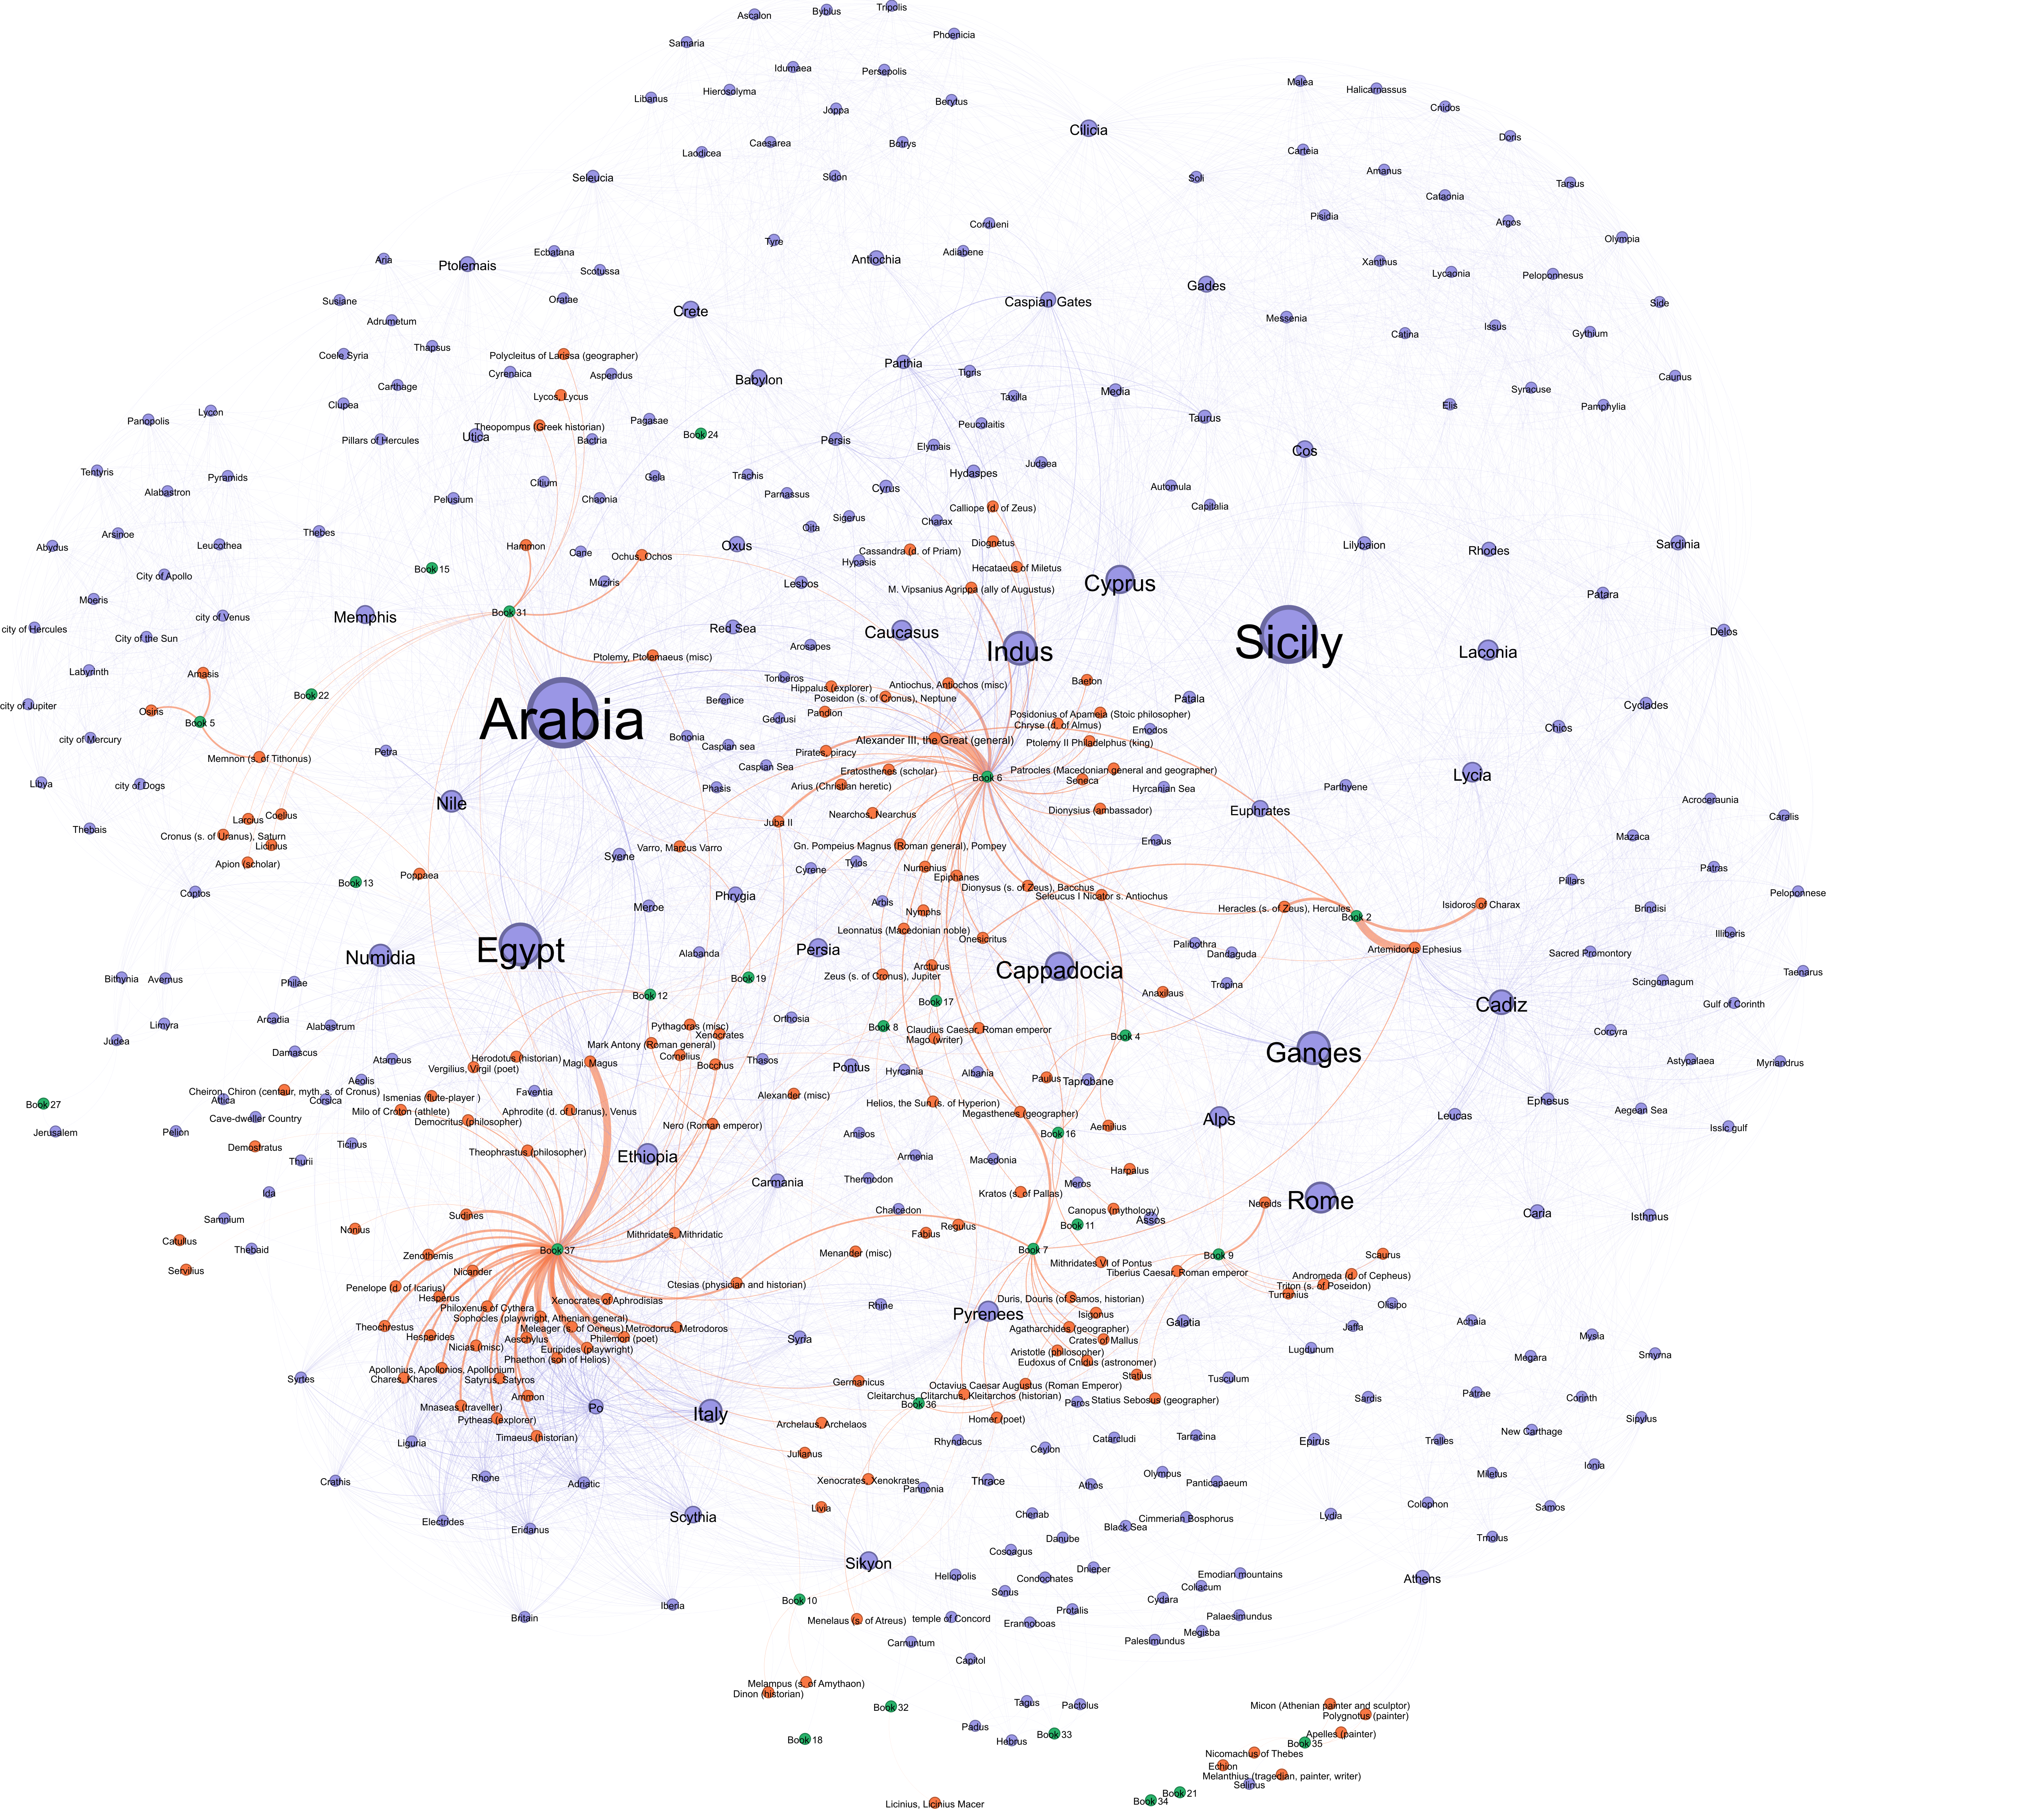
\includegraphics{NHthesis_structure_files/figure-pdf/fig-network_graph-output-1.png}

}

\caption{\label{fig-network_graph}Place/person/book number network of
India-related content in \emph{Natural History}}

\end{figure}

There are relatively large nodes of place names found in the graph,
implying they are discussed closely with ``India''. These large nodes
can be categorised as in four geographical regions: Red Sea Region:
(``Arabia'', ``Egypt''); Mediterranean Region: (``Sicily'', ``Rome'',
``Cyprus''); Asia Minor: (``Cappadocia''), and Indian Region:
(``Ganges'', ``Indus'').

As no person name appears in large size as having a high centrality in
the network, there is no central person discussed in the India-related
context in the work.

Among the large place name nodes, Arabia apperars to be the largest one,
and is found often being mentioned simultaneously with India. For
instance:

\begin{quote}
13.28.1 ``Ethiopia, which is on the borders of Egypt, has virtually no
remarkable trees except the wool-tree, like the one described among the
trees of \hl{India} and \hl{Arabia}.''
\end{quote}

\begin{quote}
22.56.1 ``I myself shall not touch upon drugs imported from \hl{India}
and \hl{Arabia} or from the outer world.''
\end{quote}

In contrast, the pattern is not found in other relatively large-sized
place name nodes outside Indian region.

This close association between India and Arabia not only attributes to
Arabia's position in the middle of the route from Rome to India, also
reflects the similar role played by both areas as the importers of
luxurious and exotic commodities, as well as geographical contrast to
the Mediterranean.

The two closely connected place names linked to ``India'', situated
within the country itself, are ``Indus'' and ``Ganges''. These names
represent the two largest rivers and vital lifelines in India. In
\emph{Natural History}, Pliny dedicated exclusive chapters to each river
in book 6, underscoring their significance in the scope of the work.

``Indus'' and ``Ganges'' are further selected as the centric node
(hidden from the graph) for filtering the entities that directly connect
to them.

Figure~\ref{fig-network_indus} shows the book, person and place names
that cluster around ``Indus'' in the India-related text. It shows that
Arabia and Egypt are the two most connected places when ``Indus'' is
mentioned, and it is mentioned in books 2, 6, 12, 19, 24, 37. Compared
to Figure~\ref{fig-network_ganges}, which shows the entities centring on
``Ganges'', the content related to ``Indus'' seems to be more
concentrated on the areas through the flow of Indus River to Arabian
Sea.

\begin{figure}

{\centering \includegraphics{NHthesis_structure_files/figure-pdf/fig-network_indus-output-1.png}

}

\caption{\label{fig-network_indus}Indus centric network of India-related
content in \emph{Natural History}}

\end{figure}

On the contrary, in the ``Ganges'' network shown in
Figure~\ref{fig-network_ganges}, although the Ganges flows eastwards to
the Bay of Bengal and is more distant from the Mediterranean than the
Indus, there are more place names of Mediterranean and adjacent regions
shown in the group, such as Sicily, Lycia, Rhodes, Patara, etc.

\begin{figure}

{\centering \includegraphics{NHthesis_structure_files/figure-pdf/fig-network_ganges-output-1.png}

}

\caption{\label{fig-network_ganges}Ganges centric network of
India-related content in \emph{Natural History}}

\end{figure}

A comparison of the texts related to these two rivers shows that the
Indus is mentioned more often as a geographical reference in the
introduction of different regions or routes, while the Ganges is
mentioned more often as the origin of special creatures or products,
such as large eels or trees and precious stones, in a context of
comparison with its counterparts in other regions.

In this case, the structural difference of a particular entity shown in
the network can lead to a more profound understanding of the target
context.

In addition, the general network graph shows two obvious clusters of
person names centred around book 6 and book 37. An enlarged snapshot of
each group is shown in Figure~\ref{fig-network_zoom_book6} (for book 6)
and Figure~\ref{fig-network_zoom_book37}.

\begin{figure}

{\centering \includegraphics{NHthesis_structure_files/figure-pdf/fig-network_zoom_book6-output-1.png}

}

\caption{\label{fig-network_zoom_book6}Clusters of Book 6 in
India-related content in \emph{Natural History}}

\end{figure}

In the cluster of book 6, the most frequently mentioned historical
figure is Alexander the Great, who holds the thickest edge curve in the
group. The mentions of Alexander the Great are related to the routes and
notes about the conquests of the Roman Empire in the Indian
subcontinent. This cluster also contains other important figures such as
`Juba II', `Ptolemy II Philadelphus', `Hippalus', `Patrocles' and `Gn.
Pompeius Magnus', who were governors and generals in ancient Rome. The
cluster also represents the scholars that Pliny frequently refers to in
the India-related narratives, such as `Seneca', `Eratosthenes' and
`Posidonius of Apameia'.

The edge curves also show how reference sources and historical and
mythological figures are linked between different books. For example,
book 6 shares the reference to ``Megasthenes'' with book 7, and shares
the mention of ``Alexander III the Great (General)'' and ``Heracles (s.
of Zeus), Hercules'' with book 2.

\begin{figure}

{\centering \includegraphics{NHthesis_structure_files/figure-pdf/fig-network_zoom_book37-output-1.png}

}

\caption{\label{fig-network_zoom_book37}Clusters of Book 37 in
India-related content in \emph{Natural History}}

\end{figure}

While in book 37, the cluster is heavily linked to renowned Greek
scholars, including ``Xenocrates'', ``Aeschylus'', ``Sudines'' and
``Zenothemis''. Additionally, there is a considerable connection with
the ``Magi'', referring to the priests of Zoroastrianism, a traditional
Persian religion, which is mentioned in the discussion about tales and
myths concerning the precious stones.

Upon closer examination, it is noteworthy that in book 37, Pliny
directly refuted these two groups with a stern critical attitude. The
Greek scholars and Magi are frequently cited as controversial subjects
in book 37, serving as a strategy for Pliny to express his own worship
of nature and the material world, as quoted in the subsequent
paragraphs.

\begin{quote}
37.11.2 ``Here is an opportunity for
\hl{exposing the falsehoods of the Greeks}.''
\end{quote}

\begin{quote}
37.14.1 ``Now I shall discuss those kinds of gemstones that are
acknowledged as such, beginning with the finest. And this shall not be
my only aim, but to the greater profit of mankind
\hl{I shall incidentally confute the abominable falsehoods of the Magi},
since in very many of their statements about gems they have gone far
beyond providing an alluring substitute for medical science into the
realms of the supernatural.''
\end{quote}

In summary, the network graphs visually portrays the interconnectivity
among the clustered entities and the selected central entities in the
narrative. This study utilizes a general network graph centered on
``India'' to reveal the closely linked places and the clustering of
historical figures, mythical gods, explorers, and scholars mentioned
across different books. Furthermore, two additional filtered networks,
with ``Indus'' and ``Ganges'' as focal points, depict structural
variations in the content about these two equally significant rivers in
India as presented in \emph{Natural History}.

The exploration could be extended to include additional entity types
such as animals, events and ethnic groups in the network to obtain a
more nuanced distance map and entity clustering, revealing more
dimensions of content structure.

\newpage

\hypertarget{sec-conclusions}{%
\section{Conclusions}\label{sec-conclusions}}

\hypertarget{comprehension-of-india-in-the-narrative}{%
\subsection{Comprehension of ``India'' in the
narrative}\label{comprehension-of-india-in-the-narrative}}

Guided by the research questions of ``How is India described, and how is
the information about India structured in the work?'', the above
analysis with different methods, including word frequency and
collocation analysis, topic modelling, and network analysis, with an
integration of close reading to the textual contet, comprise a
comprehension of ``India'' in the narrative of \emph{Natural History}.

In general, India is considered a significant geographical contrast to
the Roman Empire and the Mediterranean. India is often mentioned for
comparison in descriptions of landscapes, expeditions, navigation or
trading routes, and origins of natural creatures and elements of other
locations. The names of the rivers in the India, including some
tributaries, are highlighted as references. India's role as a major
trading partner is also significant in the narrative, as it frequently
imports rare and precious treasures into the Mediterranean.

The content relating to India potentially themed in three topics which
can be illustrated in more details by closely examining the text. The
two dominant topics cover the geographical and social conditions of
Indian nations as well as stones that are originated or produced in
India. Within the topic about general introduction to India, other than
addressing it as an origin of numerous marvels, Pliny also incidentally
mentioned the epic tales and history related to the conquest of India,
suggesting an imperial perspective of the work. And in the less
prominent topic, which focused on merchandise trade, Pliny criticised
human greed and the unnecessary interference with nature that it
represents, which echoes his Stoic view of the relationship between
nature and the human world.

A network of place names, person names, and book numbers associated with
India has been created to visually represent patterns of content and
clusters of emphasis. This network highlights the mention of place names
from the Red Sea region, the Mediterranean region, Asia Minor, as well
as the Indus and Ganges rivers - two main rivers within the country, in
the Indian context. A closer examination of the network centred on these
rivers reveals a structural distinction. Pliny frequently refers to the
Indus as a geographical marker, while the Ganges often serves as a point
of comparison for the origin of products with the Mediterranean. In
addition, specific historical figures and referencing scholars tend to
cluster around different books. It is notable that Magi and Greek
scholars played a significant role as disproving subjects in the person
name cluster of book 37, which helped Pliny express his Stoic advocacy
of worshipping the natural and material world.

In summary, in Pliny's unintentional portrait, India showed its complex
figure as a geographical contrast, an origin of marvels and treasures, a
major trading partner, and a context of unnecessary luxurious pursuit of
Pliny's contemporary that he debated against in the scope of
\emph{Natural History}.

\hypertarget{distant-reading-as-a-method}{%
\subsection{Distant reading as a
method}\label{distant-reading-as-a-method}}

The attempt of employing several distant reading methods for a research
of classical text in this study has, to a certain extent, achieved a
response to the research question.

From identifying the research question to conducting analysis of the
designated text, the distant reading methods have provided valuable
insights and enriched information. However, as demonstrated in the topic
modelling section of the data analysis, it is crucial to integrate close
reading in interpreting the results obtained through distant reading.

Besides, comprehensive checks are essential to ensure the completeness
and validity of data before proceeding with the analysis techniques
mentioned. Converting complex textual content into structured data in a
tabular format requires meticulous attention to detail, as any omissions
or inaccuracies in the dataset can significantly impact subsequent
outputs and their representation.

Another benefit of adopting the distant reading approaches is that the
output dataset can be repurposed for further investigations. Together
with this thesis, the following dataset and outputs are available on the
\href{https://github.com/lizaodawn/NH_thesis}{GitHub repository} for
future use:

\begin{enumerate}
\def\labelenumi{\arabic{enumi}.}
\item
  Dataset of Indian place names mentioned in \emph{Natural Hisoty} with
  the corresponding textual passages (scraped from TOPOSText with
  supplemented mannual annotations)
\item
  Dataset of geographical names menttioned in \emph{Natural History}
  with the corresponding textual passages (scraped from TOPOSText)
\item
  Corpus files containing textual passages relevant to India from
  \emph{Natural History}
\item
  Network graph featuring connections among place names, person names,
  and book numbers pertaining to India-related content within
  \emph{Natural History}
\end{enumerate}

In addition, this thesis has been effectively presented by integrating
\href{https://quarto.org/}{Quarto} with
\href{https://jupyter.org/}{Jupyter} Notebook. A cohesive presentation
across HTML and PDF formats has been achieved by embedding YAML metadata
and markdown language within the notebook. The HTML rendering makes it
easy to distribute interactive maps and graphics on the web, providing a
flexible approach to sharing research results.

\hypertarget{reflection-and-limitation}{%
\subsection{Reflection and limitation}\label{reflection-and-limitation}}

Although considerable effort has been put into conducting a
comprehensive study for this thesis, there are certain limitations
within the data preprocessing and parameter tuning phases that could be
improved.

During the data preparation phase, it was discovered that Indian place
names sourced from TOPOSText were incomplete and required manual
validation. As a result, about 24\% of the original dataset was
supplemented after validation. Although these additional annotations
have been merged into the dataset containing all the place names, there
may still be missing identifications of places outside the predefined
coordinate range for India. However, manual validation and
supplementation of such cases require a significant amount of time and
effort, which was not feasible at the scale of this study. If possible,
a similar supplementation process for all place names could improve the
completeness of the dataset and promote greater contextual consistency
for the study.

And for the topic modelling section, the parameter setting of topic
number was determined through a validation process based on the
coherence score comparison. Further fine-tuning of the model could be
achieved through additional validation of parameters and broader
comparisons. Adopting this comprehensive approach would improve the
robustness of the topic modelling outcomes.

Due to time constraints, the network analysis only incorporated person
names as an additional entity node. By encompassing more entity types,
like animals, events, and ethnic groups, available through TOPOSText
annotations, deeper insight into the content's structural dynamics could
be gained by expanding this analysis. This remains to improve if the
study continues to progress. Moreover, the presentation of the network
graphs could be enhanced by exploring alternative platforms that offer
greater interactivity. A preferable approach involves creating graphs
that can be easily zoomed between various clusters and filtered based on
different node types. This interactivity would improve the accessibility
and usability of the graph's visualisation.

\newpage

\hypertarget{references}{%
\section*{References}\label{references}}
\addcontentsline{toc}{section}{References}

\bigskip

\hypertarget{refs}{}
\begin{CSLReferences}{1}{0}
\leavevmode\vadjust pre{\hypertarget{ref-akbik2018coling}{}}%
Akbik, Alan, Duncan Blythe, and Roland Vollgraf. 2018. {``Contextual
String Embeddings for Sequence Labeling.''} In \emph{{COLING} 2018, 27th
International Conference on Computational Linguistics}, 1638--49.

\leavevmode\vadjust pre{\hypertarget{ref-bail}{}}%
Bail, Christopher A. n.d. {``Topic {Modeling}.''} Accessed August 3,
2023.
\url{https://cbail.github.io/textasdata/topic-modeling/rmarkdown/Topic_Modeling.html}.

\leavevmode\vadjust pre{\hypertarget{ref-barber}{}}%
Barber, Jordan. n.d. {``Latent {Dirichlet} {Allocation} ({LDA}) with
{Python}.''} Accessed March 15, 2023.
\url{https://rstudio-pubs-static.s3.amazonaws.com/79360_850b2a69980c4488b1db95987a24867a.html}.

\leavevmode\vadjust pre{\hypertarget{ref-beagon1996}{}}%
Beagon, Mary. 1996. {``Nature and Views of Her Landscapes in {Pliny} the
{Elder}.''} In \emph{Human {Landscapes} in {Classical} {Antiquity}},
285--309. Routledge.

\leavevmode\vadjust pre{\hypertarget{ref-beagon2011}{}}%
---------. 2011. {``Chapter {Five}. {The} {Curious} {Eye} {Of} {The}
{Elder} {Pliny}.''} In \emph{Pliny the {Elder}: {Themes} and
{Contexts}}, 71--88. Brill.
\url{https://brill.com/display/book/edcoll/9789004210073/Bej.9789004202344.i-248_006.xml}.

\leavevmode\vadjust pre{\hypertarget{ref-fantoli2022}{}}%
Fantoli, Margherita. 2022. {``Statistics and Linguistics: Can We Tell
Something More about {Pliny} the {Elder}?''}
\url{https://classics-at.chs.harvard.edu/statistics-and-linguistics-can-we-tell-something-more-about-pliny-the-elder/}.

\leavevmode\vadjust pre{\hypertarget{ref-healy1999}{}}%
Healy, John F. 1999. \emph{Pliny the {Elder} on Science and Technology}.
Oxford: university press.

\leavevmode\vadjust pre{\hypertarget{ref-kapadia2022}{}}%
Kapadia, Shashank. 2022. {``Topic {Modeling} in {Python}: {Latent}
{Dirichlet} {Allocation} ({LDA}).''} \emph{Medium}.
\url{https://towardsdatascience.com/end-to-end-topic-modeling-in-python-latent-dirichlet-allocation-lda-35ce4ed6b3e0}.

\leavevmode\vadjust pre{\hypertarget{ref-lao2016}{}}%
Lao, Eugenia. 2016. {``Taxonomic {Organization} in {Pliny}'s {Natural}
{History}.''} In \emph{Greek and {Roman} Poetry, the {Elder} {Pliny}},
edited by Francis Cairns and Roy Gibson, 209--46. Papers of the
{Langford} {Latin} {Seminar} 16. Prenton: Francis Cairns Publications.

\leavevmode\vadjust pre{\hypertarget{ref-murphy2003}{}}%
Murphy, Trevor. 2003. {``11. Pliny{'}s Naturalis Historia: The Prodigal
Text.''} In, 301--22. BRILL.
\url{https://doi.org/10.1163/9789004217157_012}.

\leavevmode\vadjust pre{\hypertarget{ref-naas2002}{}}%
Naas, Valérie. 2002. \emph{Le Projet Encyclopédique de {Pline}
l'{Ancien}}. Collection de l'école Française de {Rome} 303. Rome: Ecole
française de Rome.

\leavevmode\vadjust pre{\hypertarget{ref-naas2011}{}}%
---------. 2011. {``Chapter {Four}. {Imperialism}, {Mirabilia}, {And}
{Knowledge}: {Some} {Paradoxes} {In} {The} {Naturalis} {Historia}.''} In
\emph{Pliny the {Elder}: {Themes} and {Contexts}}, 57--70. Brill.
\url{https://brill.com/display/book/edcoll/9789004210073/Bej.9789004202344.i-248_005.xml}.

\leavevmode\vadjust pre{\hypertarget{ref-neelis2011}{}}%
Neelis, J. 2011. {``Chapter {Three}. {Trade} {Networks} {In} {Ancient}
{South} {Asia}.''} In \emph{Early {Buddhist} {Transmission} and {Trade}
{Networks}}, 183--228. Brill.
\url{https://brill.com/display/book/9789004194588/Bej.9789004181595.i-372_004.xml}.

\leavevmode\vadjust pre{\hypertarget{ref-pinkster2005}{}}%
Pinkster, Harm. 2005. {``The {Language} of {Pliny} the {Elder}.''}
\emph{Journal of Asthma - J ASTHMA} 129 (November): 239--56.
\url{https://doi.org/10.5871/bacad/9780197263327.003.0011}.

\leavevmode\vadjust pre{\hypertarget{ref-pollard2009}{}}%
Pollard, Elizabeth Ann. 2009. {``Pliny's {Natural} {History} and the
{Flavian} {Templum} {Pacis}: {Botanical} {Imperialism} in
{First}-{Century} {C}. {E}. {Rome}.''} \emph{Journal of World History}
20 (3): 309--38. \url{https://www.jstor.org/stable/40542802}.

\leavevmode\vadjust pre{\hypertarget{ref-roller2022}{}}%
Roller, D. W. 2022. {``Introduction.''} In \emph{A {Guide} to the
{Geography} of {Pliny} the {Elder}}, 1--14. Cambridge: Cambridge
University Press. \url{https://doi.org/10.1017/9781108693660.003}.

\leavevmode\vadjust pre{\hypertarget{ref-rydberg-cox2021}{}}%
Rydberg-Cox, Jeff. 2021. {``Modeling the {Sources} and {Topics} of
{Pliny}'s {Natural} {History}.''} \emph{Umanistica Digitale}, no. 11:
217--29. \url{https://doi.org/10.6092/issn.2532-8816/12521}.

\leavevmode\vadjust pre{\hypertarget{ref-schultze2011}{}}%
Schultze, Clemence. 2011. {``Chapter {Ten}. {Encyclopaedic}
{Exemplarity} {In} {Pliny} {The} {Elder}.''} In \emph{Pliny the {Elder}:
{Themes} and {Contexts}}, 167--86. Brill.
\url{https://brill.com/display/book/edcoll/9789004210073/Bej.9789004202344.i-248_011.xml}.

\leavevmode\vadjust pre{\hypertarget{ref-szekely2006}{}}%
Székely, Melinda. 2006. {``Eastern {Trade} of the {Roman} {Empire} Based
on {Pliny} the {Elder}'s {Natural} {History}.''} \emph{Chronica} 6
(January): 199--206.
\url{https://www.proquest.com/docview/2379648941/citation/93A42D142D614235PQ/1}.

\leavevmode\vadjust pre{\hypertarget{ref-talbert2000-1}{}}%
Talbert, Richard J. A. 2000a. \emph{Barrington Atlas of the {Greek} and
{Roman} World: Map-by-Map Directory}. Princeton (N.J.): Princeton
university press.

\leavevmode\vadjust pre{\hypertarget{ref-talbert2000}{}}%
---------. 2000b. \emph{Barrington Atlas of the {Greek} and {Roman}
World.} Princeton (N.J.): Princeton university press.

\leavevmode\vadjust pre{\hypertarget{ref-tedeschi2021}{}}%
Tedeschi, Simone, Valentino Maiorca, Niccolò Campolungo, Francesco
Cecconi, and Roberto Navigli. 2021. {``WikiNEuRal: Combined Neural and
Knowledge-Based Silver Data Creation for Multilingual NER.''} In,
25212533. Punta Cana, Dominican Republic: Association for Computational
Linguistics. \url{https://aclanthology.org/2021.findings-emnlp.215}.

\leavevmode\vadjust pre{\hypertarget{ref-tran2022}{}}%
Tran, Khuyen. 2022. {``pyLDAvis: Topic Modelling Exploration Tool That
Every NLP Data Scientist Should Know.''}
\url{https://neptune.ai/blog/pyldavis-topic-modelling-exploration-tool-that-every-nlp-data-scientist-should-know}.

\leavevmode\vadjust pre{\hypertarget{ref-underwood2012}{}}%
Underwood, Ted. 2012. {``Topic Modeling Made Just Simple Enough.''}
\emph{The Stone and the Shell}.
\url{https://tedunderwood.com/2012/04/07/topic-modeling-made-just-simple-enough/}.

\end{CSLReferences}

\newpage

\hypertarget{appendix}{%
\section*{Appendix}\label{appendix}}
\addcontentsline{toc}{section}{Appendix}

\textbf{Retrieved person name with TOPOSText}

\begin{longtable}[]{@{}llll@{}}
\toprule\noalign{}
& Person\_name & ToposText\_ID & Person\_name\_concat \\
\midrule\noalign{}
\endhead
\bottomrule\noalign{}
\endlastfoot
0 & Onesicritus & /people/936 & Onesicritus \\
1 & Alexander & /people/6 & Alexander III, the Great (general) \\
2 & Hercules & /people/4 & Heracles (s. of Zeus), Hercules \\
3 & Artemidorus & /people/15233 & Artemidorus Ephesius \\
4 & Isidore & /people/12410 & Isidoros of Charax \\
5 & Father Liber & /people/5 & Dionysus (s. of Zeus), Bacchus \\
6 & Paulus & /people/200 & Paulus \\
7 & Aemilius & /people/116 & Aemilius \\
8 & Amasis & /people/424 & Amasis \\
9 & Memnon & /people/1491 & Memnon (s. of Tithonus) \\
10 & Osiris & /people/187 & Osiris \\
11 & Calliope & /people/736 & Calliope (d. of Zeus) \\
12 & Antiochus & /people/14444 & Antiochus, Antiochos (misc) \\
13 & Seleucus & /people/12246 & Seleucus I Nicator s. Antiochus \\
14 & Margus & /people/3627 & Margos \\
15 & Orodes & /people/2010 & Orodes \\
16 & Crassus & /people/95 & Crassus \\
17 & Ochus & /people/748 & Ochus, Ochos \\
18 & Cyrus & /people/27 & Cyrus (kings of Persia) \\
19 & Semiramis & /people/332 & Semiramis \\
20 & Demodamas & /people/9252 & Demodamas (geographer) \\
21 & Apollo & /people/2 & Apollo (s. of Zeus) (cf Phoebus) \\
22 & Varro & /people/10949 & Varro, Marcus Varro \\
23 & Pompey & /people/7 & Gn. Pompeius Magnus (Roman general), Pompey \\
24 & Mithridatic & /people/44 & Mithridates, Mithridatic \\
25 & Chryse & /people/2968 & Chryse (d. of Almus) \\
26 & Hecataeus & /people/13921 & Hecataeus of Miletus \\
27 & Eratosthenes & /people/132 & Eratosthenes (scholar) \\
28 & Agrippa & /people/91 & M. Vipsanius Agrippa (ally of Augustus) \\
29 & Posidonius & /people/457 & Posidonius of Apameia (Stoic
philosopher) \\
30 & Patrocles & /people/12353 & Patrocles (Macedonian general and
geographer) \\
31 & Megasthenes & /people/1316 & Megasthenes (geographer) \\
32 & Dionysius & /people/14629 & Dionysius (ambassador) \\
33 & Philadelphus & /people/8222 & Ptolemy II Philadelphus (king) \\
34 & Seneca & /people/12005 & Seneca \\
35 & Diognetus & /people/15427 & Diognetus \\
36 & Baeton & /people/17484 & Baeton \\
37 & Strength & /people/3102 & Kratos (s. of Pallas) \\
38 & Jupiter & /people/1 & Zeus (s. of Cronus), Jupiter \\
39 & Claudius & /people/299 & Claudius Caesar, Roman emperor \\
40 & Annius & /people/1125 & Annius \\
41 & Sun & /people/180 & Helios, the Sun (s. of Hyperion) \\
42 & Canopus & /people/2757 & Canopus (mythology) \\
43 & Arius & /people/1934 & Arius (Christian heretic) \\
44 & Juba & /people/13985 & Juba II \\
45 & Nearchus & /people/14880 & Nearchos, Nearchus \\
46 & Leonnatus & /people/1114 & Leonnatus (Macedonian noble) \\
47 & Nymphs & /people/159 & Nymphs \\
48 & Arcturus & /people/632 & Arcturus \\
49 & pirates & /people/10975 & Pirates, piracy \\
50 & Hippalus & /people/6538 & Hippalus (explorer) \\
51 & Pandion & /people/507 & Pandion \\
52 & Cassandra & /people/631 & Cassandra (d. of Priam) \\
53 & Neptune & /people/25 & Poseidon (s. of Cronus), Neptune \\
54 & Epiphanes & /people/1219 & Epiphanes \\
55 & Numenius & /people/1005 & Numenius \\
56 & Ctesias & /people/485 & Ctesias (physician and historian) \\
57 & Eudoxus & /people/12988 & Eudoxus of Cnidus (astronomer) \\
58 & Homer & /people/9 & Homer (poet) \\
59 & Aristotle & /people/46 & Aristotle (philosopher) \\
60 & Isigonus & /people/14546 & Isigonus \\
61 & Crates & /people/13722 & Crates of Mallus \\
62 & Agatharchides & /people/1500 & Agatharchides (geographer) \\
63 & Clitarchus & /people/1776 & Cleitarchus, Clitarchus, Kleitarchos
(historian) \\
64 & Duris & /people/1019 & Duris, Douris (of Samos, historian) \\
65 & Germanicus & /people/2619 & Germanicus \\
66 & Herodotus & /people/133 & Herodotus (historian) \\
67 & Metrodorus & /people/435 & Metrodorus, Metrodoros \\
68 & Regulus & /people/512 & Regulus \\
69 & Ptolemy & /people/21 & Ptolemy, Ptolemaeus (misc) \\
70 & Tiberius & /people/370 & Tiberius Caesar, Roman emperor \\
71 & Triton & /people/664 & Triton (s. of Poseidon) \\
72 & Nereids & /people/590 & Nereids \\
73 & Augustus & /people/8 & Octavius Caesar Augustus (Roman Emperor) \\
74 & Turranius & /people/5299 & Turranius \\
75 & Andromeda & /people/691 & Andromeda (d. of Cepheus) \\
76 & Scaurus & /people/725 & Scaurus \\
77 & Statius & /people/594 & Statius \\
78 & Sebosus & /people/15284 & Statius Sebosus (geographer) \\
79 & Dinon & /people/2046 & Dinon (historian) \\
80 & Melampus & /people/790 & Melampus (s. of Amythaon) \\
81 & Democritus & /people/139 & Democritus (philosopher) \\
82 & Virgil & /people/118 & Vergilius, Virgil (poet) \\
83 & Nero & /people/66 & Nero (Roman emperor) \\
84 & Mithridates & /people/14100 & Mithridates VI of Pontus \\
85 & Fabius & /people/101 & Fabius \\
86 & Chiron & /people/1086 & Cheiron, Chiron (centaur, myth. s. of
Cronus) \\
87 & Poppaea & /people/3075 & Poppaea \\
88 & Theophrastus & /people/129 & Theophrastus (philosopher) \\
89 & Harpalus & /people/477 & Harpalus \\
90 & Mago & /people/15015 & Mago (writer) \\
91 & Anaxilaus & /people/16854 & Anaxilaus \\
92 & Cleopatra & /people/2952 & Cleopatra \\
93 & Antony & /people/10 & Mark Antony (Roman general) \\
94 & Polyclitus & /people/14472 & Polycleitus of Larissa (geographer) \\
95 & Lycos & /people/2529 & Lycos, Lycus \\
96 & Theopompus & /people/121 & Theopompus (Greek historian) \\
97 & Coelius & /people/2100 & Coelius \\
98 & Apion & /people/1363 & Apion (scholar) \\
99 & Saturn & /people/43 & Cronus (s. of Uranus), Saturn \\
100 & Larcius & /people/12061 & Larcius \\
101 & Licinius & /people/232 & Licinius \\
102 & Hammon & /people/2204 & Hammon \\
103 & Licinius Macer & /people/14785 & Licinius, Licinius Macer \\
104 & Polygnotus & /people/1079 & Polygnotus (painter) \\
105 & Micon & /people/1672 & Micon (Athenian painter and sculptor) \\
106 & Apelles & /people/460 & Apelles (painter) \\
107 & Aetion & /people/13110 & Echion \\
108 & Melanthius & /people/921 & Melanthius (tragedian, painter,
writer) \\
109 & Nicomachus & /people/14661 & Nicomachus of Thebes \\
110 & Menelaus & /people/53 & Menelaus (s. of Atreus) \\
111 & Xenocrates & /people/365 & Xenocrates, Xenokrates \\
112 & Pythagoras & /people/14445 & Pythagoras (misc) \\
113 & Cornelius & /people/89 & Cornelius \\
114 & Bocchus & /people/1442 & Bocchus \\
115 & Xenocrates & /people/14598 & Xenocrates \\
116 & Sudines & /people/4698 & Sudines \\
117 & Livia & /people/589 & Livia \\
118 & Phaethon & /people/273 & Phaethon (son of Helios) \\
119 & Aeschylus & /people/174 & Aeschylus \\
120 & Philoxenus & /people/14212 & Philoxenus of Cythera \\
121 & Euripides & /people/75 & Euripides (playwright) \\
122 & Nicander & /people/14906 & Nicander \\
123 & Satyrus & /people/397 & Satyrus, Satyros \\
124 & Apollonius & /people/333 & Apollonius, Apollonios, Apollonium \\
125 & Chares & /people/462 & Chares, Khares \\
126 & Ammon & /people/577 & Ammon \\
127 & Philemon & /people/638 & Philemon (poet) \\
128 & Zenothemis & /people/17964 & Zenothemis \\
129 & Pytheas & /people/678 & Pytheas (explorer) \\
130 & Timaeus & /people/12984 & Timaeus (historian) \\
131 & Nicias & /people/12472 & Nicias (misc) \\
132 & Theochrestus & /people/8397 & Theochrestus \\
133 & Xenocrates & /people/15164 & Xenocrates of Aphrodisias \\
134 & Mnaseas & /people/1566 & Mnaseas (traveller) \\
135 & Penelope & /people/264 & Penelope (d. of Icarius) \\
136 & Hesperides & /people/597 & Hesperides \\
137 & Hesperus & /people/1702 & Hesperus \\
138 & Sophocles & /people/131 & Sophocles (playwright, Athenian
general) \\
139 & Meleager & /people/315 & Meleager (s. of Oeneus) \\
140 & Julianus & /people/732 & Julianus \\
141 & Archelaus & /people/113 & Archelaus, Archelaos \\
142 & Nonius & /people/2174 & Nonius \\
143 & Catullus & /people/1881 & Catullus \\
144 & Servilius & /people/213 & Servilius \\
145 & Ismenias & /people/860 & Ismenias (flute-player ) \\
146 & Demostratus & /people/1995 & Demostratus \\
147 & Menander & /people/14475 & Menander (misc) \\
148 & Magi & /people/12091 & Magi, Magus \\
149 & Petra & /people/2341 & Petra \\
150 & Venus & /people/15 & Aphrodite (d. of Uranus), Venus \\
151 & Milo & /people/351 & Milo of Croton (athlete) \\
152 & Alexander & /people/13 & Alexander (misc) \\
\end{longtable}

\newpage

\textbf{Retrieved person name with Wiki}

*Retrieved names without a comment are validated as person names

\begin{longtable}[]{@{}lll@{}}
\toprule\noalign{}
& wiki\_PER\_name\_tag & Comment \\
\midrule\noalign{}
\endhead
\bottomrule\noalign{}
\endlastfoot
0 & Onesicritus & NaN \\
1 & Alexander & NaN \\
2 & Artemidorus & NaN \\
3 & Isidore & NaN \\
4 & Father Liber & NaN \\
5 & Hercules & NaN \\
6 & Paulus Aemilius & NaN \\
7 & Amasis & NaN \\
8 & Alexander the Great & NaN \\
9 & Antiochus & NaN \\
10 & Seleucus & NaN \\
11 & M & should be M. Varro \\
12 & Varro & NaN \\
13 & Amometus & NaN \\
14 & Hecataeus & NaN \\
15 & Eratosthenes & NaN \\
16 & Agrippa & NaN \\
17 & Posidonius & NaN \\
18 & Patrocles & NaN \\
19 & Megasthenes & NaN \\
20 & Dionysius & NaN \\
21 & Philadelphus & NaN \\
22 & Seneca & NaN \\
23 & Diognetus & NaN \\
24 & Baeton & NaN \\
25 & Seleucus Nicator & NaN \\
26 & Bacchus & NaN \\
27 & Jupiter & NaN \\
28 & Claudius & NaN \\
29 & Annius Plocamus & NaN \\
30 & Rachias & NaN \\
31 & Taprobane & NaN \\
32 & Cyrus & NaN \\
33 & Semiramis & NaN \\
34 & Juba & NaN \\
35 & Nearchus & NaN \\
36 & Leonnatus & NaN \\
37 & Pandion & NaN \\
38 & Erythras & NaN \\
39 & Epiphanes & NaN \\
40 & Ctesias & NaN \\
41 & Pompey the Great & NaN \\
42 & Liber & NaN \\
43 & Procilius & NaN \\
44 & Pompey & NaN \\
45 & Germanicus Caesar & NaN \\
46 & Herodotus & NaN \\
47 & Regulus & NaN \\
48 & Ptolemy & NaN \\
49 & Tiberius & NaN \\
50 & Triton & NaN \\
51 & Augustus & NaN \\
52 & Turranius & NaN \\
53 & Andromeda & NaN \\
54 & Marcus Scaurus & NaN \\
55 & Statius Sebosus & NaN \\
56 & Dinon & NaN \\
57 & Clitarchus & NaN \\
58 & Melampus & NaN \\
59 & Democritus & NaN \\
60 & Homer & NaN \\
61 & Virgil & NaN \\
62 & Nero & NaN \\
63 & Mithridates & NaN \\
64 & Fabius & NaN \\
65 & Chiron & NaN \\
66 & Poppaea & NaN \\
67 & Nature & Personification of nature, "in accordance with
Nature\textquotesingle s will and pleasure" \\
68 & Theophrastus & NaN \\
69 & Harpalus & NaN \\
70 & Anaxilaus & NaN \\
71 & Cleopatra & NaN \\
72 & Mark Antony & NaN \\
73 & Polyclitus & NaN \\
74 & Theopompus & NaN \\
75 & Coelius & NaN \\
76 & Apion & NaN \\
77 & Medes & location name \\
78 & Saturn & NaN \\
79 & Bryazus & NaN \\
80 & Larcius Licinius & NaN \\
81 & Licinius Macer & NaN \\
82 & Avarice & Personification in the context \\
83 & Polygnotus & NaN \\
84 & Micon & NaN \\
85 & Apelles & NaN \\
86 & Selinus & location name \\
87 & Aetion & NaN \\
88 & Melanthius & NaN \\
89 & Nicomachus & NaN \\
90 & Man & Collective Noun \\
91 & Obsius & NaN \\
92 & Menelaus & NaN \\
93 & Scius & NaN \\
94 & Xenocrates & NaN \\
95 & Pythagoras & NaN \\
96 & Cornelius Bocchus & NaN \\
97 & Sudines & NaN \\
98 & Livia & NaN \\
99 & Phaethon & NaN \\
100 & Aeschylus & NaN \\
101 & Philoxenus & NaN \\
102 & Euripides & NaN \\
103 & Nicander & NaN \\
104 & Satyrus & NaN \\
105 & Apollonius & NaN \\
106 & Chares & NaN \\
107 & Philemon & NaN \\
108 & Caesar Germanicus & NaN \\
109 & Antony & NaN \\
110 & Nonius & NaN \\
111 & Nonius Struma & NaN \\
112 & Catullus & NaN \\
113 & Servilius Nonianus & NaN \\
114 & Ismenias & NaN \\
115 & Demostratus & NaN \\
116 & Zenothemis & NaN \\
117 & Sotacus & NaN \\
118 & Menander & NaN \\
119 & Venus & NaN \\
120 & Milo & NaN \\
\end{longtable}

\newpage

\textbf{Retrieved person name with Flair}

*Retrieved names without a comment are validated as person names

\begin{longtable}[]{@{}lll@{}}
\toprule\noalign{}
& flair\_PER\_name\_tag & Comment.1 \\
\midrule\noalign{}
\endhead
\bottomrule\noalign{}
\endlastfoot
0 & Leo & Zodiac, also a person name \\
1 & Alexander & NaN \\
2 & Onesicritus & NaN \\
3 & Paulus Aemilius & NaN \\
4 & Cyrus & NaN \\
5 & SCYTHIA & location name \\
6 & Aramii & location name, appears after "the name of..." \\
7 & M. Varro & NaN \\
8 & Pompey & NaN \\
9 & Laros & location name \\
10 & Hecataeus & NaN \\
11 & Patrocles & NaN \\
12 & Alexander the Great & NaN \\
13 & Baeton & NaN \\
14 & Protalis & location name, appears after "the name of..." \\
15 & Hercules & NaN \\
16 & Patala & location name \\
17 & TAPROBANE & NaN \\
18 & Annius Plocamus & NaN \\
19 & Rachias & NaN \\
20 & SABTUL & NaN \\
21 & Daritis & location name \\
22 & Nearchus & NaN \\
23 & the "Island of the Sun" & location name \\
24 & Muza & location name, appears in "...by name" \\
25 & Barace & Ethnic group, appears in "...by name" \\
26 & Therothoae & location name, appears in "...have the name of..." \\
27 & Coele Syria & location name, appears after "the name of..." \\
28 & Tauron & NaN \\
29 & Choromandae & location name, appears after "the name of..." \\
30 & Homer & NaN \\
31 & Aristotle & NaN \\
32 & Isigonus & NaN \\
33 & Mandi & refer to locusts in the context, appears after "the name
of..." \\
34 & Megasthenes & NaN \\
35 & Duris & NaN \\
36 & Herodotus & NaN \\
37 & Regulus & NaN \\
38 & Claudius & NaN \\
39 & Ptolemy & NaN \\
40 & Marcus Scaurus & NaN \\
41 & Dinon & NaN \\
42 & Clitarchus & NaN \\
43 & Democritus & NaN \\
44 & Virgil & NaN \\
45 & the Emperor Nero & NaN \\
46 & Mago & NaN \\
47 & Cadurci & Ethnic group \\
48 & Ruteni & Ethnic group \\
49 & Varro & NaN \\
50 & Anaxilaus & NaN \\
51 & Theophrastus & NaN \\
52 & Coelius & NaN \\
53 & Licinius Macer & NaN \\
54 & Micon & NaN \\
55 & Aetion & NaN \\
56 & Melinum & name of a type of oil, appears in "which I have
called..." \\
57 & Cornelius Bocchus & NaN \\
58 & Aeschylus & NaN \\
59 & Sudines & NaN \\
60 & Sotacus & NaN \\
61 & Xenocrates & NaN \\
62 & Meleager & NaN \\
63 & Sophocles & NaN \\
64 & Caesar Germanicus & NaN \\
65 & Transpadane Gaul & location name \\
66 & Zenothemis & NaN \\
67 & Ismenias & NaN \\
68 & Magi & NaN \\
69 & Milo & NaN \\
70 & Atizoe & stone name, appears in "The Atizoe, he writes...", "he"
here refer to the Magi in the context \\
\end{longtable}



\end{document}
